
%%%%%%%%%%%%%%%%%%%%%%%%%%%%%%%%%%%%%%%%%%%%%%%%%%%%%%%%%%%%%%%%%%%%%
%% This is a (brief) model paper using the achemso class
%% The document class accepts keyval options, which should include
%% the target journal and optionally the manuscript type.
%%%%%%%%%%%%%%%%%%%%%%%%%%%%%%%%%%%%%%%%%%%%%%%%%%%%%%%%%%%%%%%%%%%%%
\documentclass[journal=jacsat,manuscript=article]{achemso}

%%%%%%%%%%%%%%%%%%%%%%%%%%%%%%%%%%%%%%%%%%%%%%%%%%%%%%%%%%%%%%%%%%%%%
%% Place any additional packages needed here.  Only include packages
%% which are essential, to avoid problems later. Do NOT use any
%% packages which require e-TeX (for example etoolbox): the e-TeX
%% extensions are not currently available on the ACS conversion
%% servers.
%%%%%%%%%%%%%%%%%%%%%%%%%%%%%%%%%%%%%%%%%%%%%%%%%%%%%%%%%%%%%%%%%%%%%
\usepackage[version=3]{mhchem} % Formula subscripts using \ce{}
\usepackage[obeyFinal]{easy-todo}
\usepackage{rotating}
%%%%%%%%%%%%%%%%%%%%%%%%%%%%%%%%%%%%%%%%%%%%%%%%%%%%%%%%%%%%%%%%%%%%%
%% If issues arise when submitting your manuscript, you may want to
%% un-comment the next line.  This provides information on the
%% version of every file you have used.
%%%%%%%%%%%%%%%%%%%%%%%%%%%%%%%%%%%%%%%%%%%%%%%%%%%%%%%%%%%%%%%%%%%%%
%%\listfiles

%%%%%%%%%%%%%%%%%%%%%%%%%%%%%%%%%%%%%%%%%%%%%%%%%%%%%%%%%%%%%%%%%%%%%
%% Place any additional macros here.  Please use \newcommand* where
%% possible, and avoid layout-changing macros (which are not used
%% when typesetting).
%%%%%%%%%%%%%%%%%%%%%%%%%%%%%%%%%%%%%%%%%%%%%%%%%%%%%%%%%%%%%%%%%%%%%
\newcommand*\mycommand[1]{\texttt{\emph{#1}}}

%%%%%%%%%%%%%%%%%%%%%%%%%%%%%%%%%%%%%%%%%%%%%%%%%%%%%%%%%%%%%%%%%%%%%
%% Meta-data block
%% ---------------
%% Each author should be given as a separate \author command.
%%
%% Corresponding authors should have an e-mail given after the author
%% name as an \email command. Phone and fax numbers can be given
%% using \phone and \fax, respectively; this information is optional.
%%
%% The affiliation of authors is given after the authors; each
%% \affiliation command applies to all preceding authors not already
%% assigned an affiliation.
%%
%% The affiliation takes an option argument for the short name.  This
%% will typically be something like "University of Somewhere".
%%
%% The \altaffiliation macro should be used for new address, etc.
%% On the other hand, \alsoaffiliation is used on a per author basis
%% when authors are associated with multiple institutions.
%%%%%%%%%%%%%%%%%%%%%%%%%%%%%%%%%%%%%%%%%%%%%%%%%%%%%%%%%%%%%%%%%%%%%
%\author{Andrew N. Other}
%\altaffiliation{A shared footnote}
%\author{Fred T. Secondauthor}
%\altaffiliation{Current address: Some other place, Othert\"own,
%Germany}
%\author{I. Ken Groupleader}
%\altaffiliation{A shared footnote}
%\email{i.k.groupleader@unknown.uu}
%\phone{+123 (0)123 4445556}
%\fax{+123 (0)123 4445557}
%\affiliation[Unknown University]
%{Department of Chemistry, Unknown University, Unknown Town}
%\alsoaffiliation[Second University]
%{Department of Chemistry, Second University, Nearby Town}
%\author{Susanne K. Laborator}
%\email{s.k.laborator@bigpharma.co}
%\affiliation[BigPharma]
%{Lead Discovery, BigPharma, Big Town, USA}
%\author{Kay T. Finally}
%\affiliation[Unknown University]
%{Department of Chemistry, Unknown University, Unknown Town}
%\alsoaffiliation[Second University]
%{Department of Chemistry, Second University, Nearby Town}

\author{Alexandru Botan}
%\affiliation{The authors are listed in alphaphetical order.}
%\affiliation{The author list is not completed.}
\affiliation[Lyon CNRS]{Institut Lumi\`ere Mati\`ere, UMR5306 Universit\'e Lyon 1-CNRS, Universit\'e de Lyon 69622 Villeurbanne, France}
%
%\author{Andrea Catte}
%\affiliation{University of East Anglia, Norwich, United Kingdom}
\author{Fernando Favela-Rosales}
\affiliation[Mexico]{Departamento de F\'isica, Centro de Investigaci\'on y de Estudios Avanzados del IPN, Apartado Postal 14-740, 07000 M\'exico D.F., M\'exico}
\author{Patrick F. J. Fuchs}
\affiliation[CNRS Paris]{Institut Jacques Monod, CNRS, Universit\'e Paris Diderot, Sorbonne Paris Cit\'e, Paris, France}
%\alsoaffiliation[Diderot University]
%{Institut Jacques Monod, CNRS UMR 7592, Universit{\'e} Paris Diderot, Sorbonne Paris Cit{\'e}, Paris, France}
\author{Matti Javanainen}
\affiliation[Tampere University of Technology]
{Department of Physics, Tampere University of Technology, Tampere, Finland}
\author{Matej Kandu\v{c}}
\affiliation[Freie Universit\"{a}t Berlin] 
{Fachbereich Physik, Freie Universitat Berlin, Berlin, Germany}
\author{Waldemar Kulig}
\affiliation[Tampere University of Technology]
{Department of Physics, Tampere University of Technology, Tampere, Finland}
\author{Antti Lamberg}
\affiliation[Kyoto University]
{Department of Chemical Engineering, Kyoto University, Kyoto, Japan}
\author{Claire Loison}
\affiliation[Lyon CNRS]{Institut Lumi\`ere Mati\`ere, UMR5306 Universit\'e Lyon 1-CNRS, Universit\'e de Lyon 69622 Villeurbanne, France}
\author{Markus S. Miettinen}
\affiliation[Freie Universit\"{a}t Berlin] 
{Fachbereich Physik, Freie Universitat Berlin, Berlin, Germany}
\author{Luca Monticelli}
\affiliation[UMR] 
{5IBCP, CNRS UMR 5086, Lyon, France}
\author{Jukka M{\"a}{\"a}tt{\"a}}
\affiliation[Aalto University]
{Aalto University, Espoo, Finland}
\author{O. H. Samuli Ollila} 
\email{samuli.ollila@aalto.fi.}
\affiliation[Aalto University]
{Aalto University, Espoo, Finland}
\author{Marius Retegan}
\affiliation[Max Planck]
{Max Planck Institute for Chemical Energy Conversion, Mulheim an der Ruhr, Germany}
\author{Tomasz Rog}
\affiliation[Tampere University of Technology]
{Department of Physics, Tampere University of Technology, Tampere, Finland}
\author{Hubert Santuz}
\affiliation[INSERM]
{INSERM, UMR\_S 1134, DSIMB, Paris, France}
\alsoaffiliation[Diderot]
{Universit\'e Paris Diderot, Sorbonne Paris Cit\'e, UMR\_S 1134, Paris, France}
\alsoaffiliation[INTS]
{Institut National de la Transfusion Sanguine (INTS), Paris, France}
\alsoaffiliation[Labex]
{Laboratoire d'Excellence GR-Ex, Paris, France}
\author{Joona Tynkkynen}
\affiliation[Tampere University of Technology]
{Department of Physics, Tampere University of Technology, Tampere, Finland}



%%%%%%%%%%%%%%%%%%%%%%%%%%%%%%%%%%%%%%%%%%%%%%%%%%%%%%%%%%%%%%%%%%%%%
%% The document title should be given as usual. Some journals require
%% a running title from the author: this should be supplied as an
%% optional argument to \title.
%%%%%%%%%%%%%%%%%%%%%%%%%%%%%%%%%%%%%%%%%%%%%%%%%%%%%%%%%%%%%%%%%%%%%
\title[An \textsf{achemso} demo]
  {Towards atomistic resolution structure of phosphatidylcholine glycerol backbone and choline headgroup at different ambient conditions\footnote{Publication about results presented in the NMRlipids project}}

%%%%%%%%%%%%%%%%%%%%%%%%%%%%%%%%%%%%%%%%%%%%%%%%%%%%%%%%%%%%%%%%%%%%%
%% Some journals require a list of abbreviations or keywords to be
%% supplied. These should be set up here, and will be printed after
%% the title and author information, if needed.
%%%%%%%%%%%%%%%%%%%%%%%%%%%%%%%%%%%%%%%%%%%%%%%%%%%%%%%%%%%%%%%%%%%%%
\abbreviations{IR,NMR,UV}
\keywords{American Chemical Society, \LaTeX}

%%%%%%%%%%%%%%%%%%%%%%%%%%%%%%%%%%%%%%%%%%%%%%%%%%%%%%%%%%%%%%%%%%%%%
%% The manuscript does not need to include \maketitle, which is
%% executed automatically.
%%%%%%%%%%%%%%%%%%%%%%%%%%%%%%%%%%%%%%%%%%%%%%%%%%%%%%%%%%%%%%%%%%%%%
\begin{document}

%%%%%%%%%%%%%%%%%%%%%%%%%%%%%%%%%%%%%%%%%%%%%%%%%%%%%%%%%%%%%%%%%%%%%
%% The "tocentry" environment can be used to create an entry for the
%% graphical table of contents. It is given here as some journals
%% require that it is printed as part of the abstract page. It will
%% be automatically moved as appropriate.
%%%%%%%%%%%%%%%%%%%%%%%%%%%%%%%%%%%%%%%%%%%%%%%%%%%%%%%%%%%%%%%%%%%%%
\begin{tocentry}

Some journals require a graphical entry for the Table of Contents.
This should be laid out ``print ready'' so that the sizing of the
text is correct.

Inside the \texttt{tocentry} environment, the font used is Helvetica
8\,pt, as required by \emph{Journal of the American Chemical
Society}.

The surrounding frame is 9\,cm by 3.5\,cm, which is the maximum
permitted for  \emph{Journal of the American Chemical Society}
graphical table of content entries. The box will not resize if the
content is too big: instead it will overflow the edge of the box.

This box and the associated title will always be printed on a
separate page at the end of the document.

\end{tocentry}

%%%%%%%%%%%%%%%%%%%%%%%%%%%%%%%%%%%%%%%%%%%%%%%%%%%%%%%%%%%%%%%%%%%%%
%% The abstract environment will automatically gobble the contents
%% if an abstract is not used by the target journal.
%%%%%%%%%%%%%%%%%%%%%%%%%%%%%%%%%%%%%%%%%%%%%%%%%%%%%%%%%%%%%%%%%%%%%
\begin{abstract}
Phospholipids are essential building blocks of biological membranes.
Despite of vast amount of accurate experimental data, the atomistic resolution structures sampled by the glycerol backbone and choline headgroup
in phoshatidylcholine bilayers are not known. Atomistic resolution molecular dynamics simulations model 
would automatically resolve the structures giving an interpretation of experimental results, if the model
reproduced the experimental data. 
In the present work we simulate phosphatidylcholine (PC) lipid bilayers with 13 different
atomistic models, and we compare simulations with experiments (in fully hydrated conditions) in terms of C--H bond vector order
parameters for the glycerol backbone and choline headgroups. 
We show that this comparison can be used to judge the atomistic resolution structural accuracy of the models,
thus allowing the usage of molecular dynamics simulations to interpret the structures of biomolecules in 
biologically relevant conditions from NMR experiments. Further, we review previous experimental
data for dehydrated lipid bilayers and cholesterol containing bilayers, and interpretate it with simulations.
The interpretation suggest that the increased choline order parameters indicate P--N vector tilting more parallel to membrane,
and that cholesterol induces only minor changes to the glycerol backbone structure.
%None of the current models is not accurately enough to resolve the structure with experimental accuracy.
%However, closer inspection of three best performing models (CHARMM36, GAFFlipid and MacRog) suggest
%that improvements in the sampled dihedral angle distributions would potentilly lead to the model which
%would resolve the structure. Despite of the inaccuracy in the fully hydrated
%structures, the response to dehydration, i.e. the tilting of the P--N vector more parallel to membrane normal, 
%is qualitatively correct in all models. The CHARMM36 and MacRog models describe the interactions
%between lipids and cholesterol better than the Berger/H\"oltje model.
This work has been done as an open collaboration by using the \url{nmrlipids.blogspot.fi} as an
communication platform. All the scientific contributions have been done through the blog and
are publicly available. In addition, almost all simulation trajectories and files are made available
in the Zenodo community \url{https://zenodo.org/collection/user-nmrlipids} which has became the most extensive
publicly available collection of molecular dynamics simulation trajectories of lipid bilayers.
\end{abstract}

%%%%%%%%%%%%%%%%%%%%%%%%%%%%%%%%%%%%%%%%%%%%%%%%%%%%%%%%%%%%%%%%%%%%%
%% Start the main part of the manuscript here.
%%%%%%%%%%%%%%%%%%%%%%%%%%%%%%%%%%%%%%%%%%%%%%%%%%%%%%%%%%%%%%%%%%%%%


\section{Introduction}

Phospholipids containing various polar headgroups and acyl chains are essential building blocks of 
biological membranes. Lamellar phospholipid bilayer structures have been widely studied with various experimental 
and theoretical techniques as a simple model for cellular membranes~\cite{lipowsky95,tieleman97,klauda08,edholm08,tieleman10,piggot12,rabinovich13,marsh13}. 
Phospholipid molecules are composed of hydrophobic acyl chains which are connected by a glycerol backbone to a hydrophilic headgroup.
See Fig.~\ref{POPCstructure} for the structure of 1-palmitoyl-2-oleoylphosphatidylcholine (POPC).
The behaviour of the acyl chains in a lipid bilayer is relatively well understood~\cite{Israelachvili80,lipowsky95,tieleman97,klauda08,edholm08,tieleman10,marsh13}. 
The conformations sampled by the glycerol backbone and choline in a fluid bilayer are, however, not fully 
resolved since even the most accurate scattering and Nuclear Magnetic Resonance (NMR)
techniques give only a set of values that the structure has to fulfil, but
there is no unique way to derive the actual structure from them~\cite{seelig77b,skarjune79,Israelachvili80,jacobs80,davis83,strenk85,akutsu91,hong95b,hong96,semchyschyn04}.
Some structural details have been extracted from crystal structure, $^1$H NMR studies and Raman spectroscopy~\cite{hauser80,hauser81,hauser81b,akutsu81b,pascher92,hauser88,marsh06}
but general consensus about the structures sampled in the fluid state have not been reached~\cite{seelig77b,skarjune79,Israelachvili80,jacobs80,davis83,strenk85,hauser88,akutsu91,hong95b,hong96,semchyschyn04,marsh06}. 
On the other hand, the structural parameters for the glycerol backbone are similar for various biologically
relevant lipid species (phosphatidylcholine (PC), phosphatidylethanolamine (PE) and phosphatidylglycerol (PG)) 
in various environments~\cite{gally81} and the structural parameters for the headgroup choline structures are similar in model membranes and
real cells (mouse fibroblast L-M cell)~\cite{scherer87}.
Thus, the solution of phosphatidylcholine glycerol backbone and choline structures would be 
useful for understanding a wide range of different biological membranes.

Classical atomistic molecular dynamics simulations have been widely used to study  
lipid bilayers~\cite{tieleman97,klauda08,edholm08,tieleman10,piggot12,rabinovich13}. As these models provide an atomistic
resolution description of the whole lipid molecule, they have potential to solve the glycerol backbone and 
headgroup structures. In particular, the experimental C--H bond order parameters for the glycerol backbone 
(g$_1$, g$_2$ and g$_3$) and choline ($\alpha$ and $\beta$) segments (see Fig.~\ref{POPCstructure} for definitions) are among the main parameters used in
attempts to derive lipid structures from experimental data~\cite{seelig77b,skarjune79,jacobs80,davis83,akutsu91,hong95b,semchyschyn04}.
These parameters are also routinely compared between experiments and simulations for the acyl chains~\cite{tieleman97,klauda08,edholm08,tieleman10,piggot12}.
Thus, the structures sampled in a simulation model that reproduces these and other experimental parameters, automatically
give an interpretation of the experiments. In other words they can be considered as reasonable atomistic resolution descriptions of
the behavior of lipid molecules in a bilayer.

The glycerol backbone and choline headgroup order parameters have been compared between simulations and experiments
in some studies~\cite{shinoda97,hogberg08,castro08,klauda10,kapla12,dickson12,poger12,ferreira13,chowdhary13,maciejewski14}, 
however much less frequently than for the acyl  chains~\cite{tieleman97,klauda08,edholm08,tieleman10,piggot12}.
The main reason is probably that the existing experimental data for the glycerol backbone
and choline headgroups is scattered over many publications and published in a format that is difficult to understand without some NMR expertise. 
In addition to the order parameters, also dihedral angles for glycerol backbone and headgroup estimated from experiments have been sometimes used to 
assess the quality of a simulation model~\cite{robinson94,essex94,kothekar96,hyvonen97,shinoda97,duong99}.

In this work we first review the most relevant experimental data for the glycerol backbone and choline headgroup order parameters
in a phosphatidylcholine lipid bilayer. Then the available atomistic resolution lipid models are carefully compared to the 
experimental data. The comparison reveals that the CHARMM36~\cite{klauda10}, GAFFlipid~\cite{dickson12} and MacRog models~\cite{maciejewski14}
have the most realistic glycerol backbone and choline structures. We also compare the glycerol backbone and choline 
structures between the most often used (Berger based) lipid model~\cite{berger97} 
%\todo{If there are no objections, we will leave the naming convention of different Berger versions as it is now.}
and the best performing models, to demonstrate that by using the 
order parameters we can distinguish the more reasonable structures from the less reasonable ones. However, none of the current models 
is accurate enough to properly resolve the atomistic resolution stuctures.

In addition to fully hydrated single component lipid bilayers, the glycerol backbone and choline order parameters
have been measured under a large number of different conditions. For example, as a function of hydration level~\cite{bechinger91,ulrich94,dvinskikh05b}, cholesterol content~\cite{brown78,ferreira13}
ion concentration~\cite{brown77,akutsu81,altenbach84,roux90,roux91}, temperature~\cite{gally75}, charged lipid content~\cite{roux90,roux91}, charged surfactant content~\cite{scherer89}, 
drug molecule concentration~\cite{browning82,kelusky84,castro08}, and protein content~\cite{roux89,kuchinka89} (listing only the publications most relevant for this work and the pioneering studies).
Awareness of the existence of this type of data allows the comparison of structural responses to varying conditions between simulations and experiments,
which can be used to validate the simulation models and to interpret the original experiments. 
In this publication we demonstrate the power of this approach for understanding the behaviour of a bilayer as a function of hydration level and cholesterol concentration.
Choline headgroup order parameters as function of ion concentration, and their relation to the ion binding affinity, are discussed elsewhere~\cite{ionpaper}.

  \begin{figure}[]
  \centering
  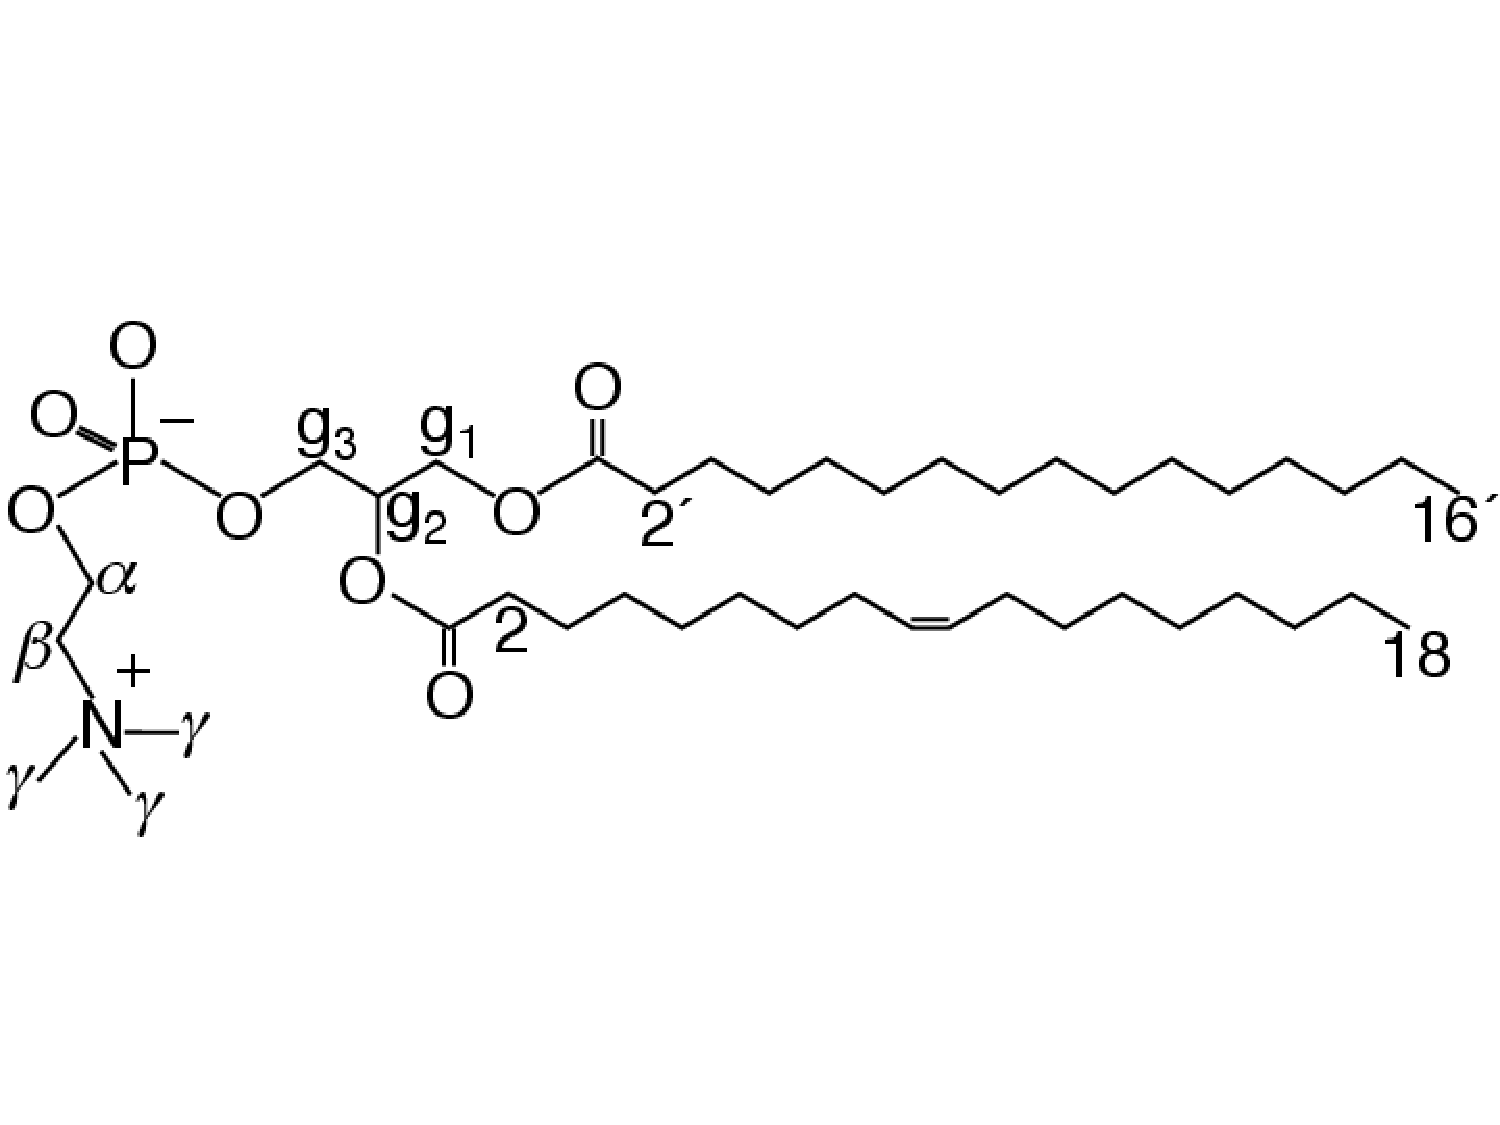
\includegraphics[width=8.6cm]{../Fig/POPCstructure.pdf}

  \caption{\label{POPCstructure}
    Chemical structure of  1-palmitoyl-2-oleoylphosphatidylcholine (POPC).}
  
\end{figure}

\section{methods}

\subsection{Open collaboration}
%\todo{Should we write more about this?}

This work has been done as an open collaboration by using \url{nmrlipids.blogspot.fi}
\todo{Current idea is that we will assign doi for the blog by using the help from  winnower administrators:
https://thewinnower.com/posts/archiving-and-aggregating-alternative-scholarly-content-dois-for-blogs.
Once done, that doi will be cited here and other places where blog content needs to be cited.} 
as a communication platform.
The approach is inspired by the Polymath project~\cite{gowers09}, however there are some essential differences. 
The present approach was started by publishing a manuscript~\cite{ollila13} discussing the glycerol backbone and choline structures 
in a Berger based model (the most used molecular dynamics simulation model for lipid bilayers).
After publishing the initial manuscript, the open invitation for further contributions and discussion through the blog was presented.
All the scientific contributions are done publicly through the blog and all contributors were offered coauthorship
according to the guidelines defined in the beginning of the project\todo{Citation to the On Credits in the blog here}. 
The acception of authorship is based on the self-assesment of the authors' scientific contribution to the project.
The contributions from each author are summarized in the Supplementary Information. %(the location depends on the journal probably).

Almost all simulation data, including running parameters for reprocution and trajectories for further analysis, are collected
to the nmrlipids community in Zenodo file repository \url{https://zenodo.org/collection/user-nmrlipids}.
Thus, besides the main topic of this manuscript we present the most extensive available collection of simulations trajectories
for lipid bilayers, which opens up numerous possiblities for different analyses with much less effort than previously required.
Furher information, e.g. scripts, figures and manuscript text files, are available in the GitHub 
organization \url{https://github.com/NMRlipids} \todo{Doi will be assigned to the GitHub repository before submission}.


\subsection{Order parameters from experiments}\label{expORDp}
The order parameter of a hydrocarbon C--H vector is defined as 
\begin{equation}\label{orderP}
S_{{\rm CH}}=\frac{1}{2}\langle 3 \cos^2 \theta-1 \rangle,
\end{equation} 
where the angle brackets denote an ensemble average over the sampled conformations, and $\theta$ is the angle between the C--H bond and the membrane normal.
The absolute values of order parameters can be measured by detecting quadrupolar splitting with $^2$H NMR~\cite{seelig77c} or by detecting dipolar 
splitting with $^1$H-$^{13}$C NMR~\cite{hong95a,gross97,dvinskikh05a,ferreira13}. The measurements are based on
different physical interactions and also the connection between order parameters and quadrupolar or dipolar splitting
are different. The absolute values of order parameters from the measured quadrupolar splitting $\Delta \nu_Q$ ($^2$H NMR) are calculated using 
the equation $|S_{{\rm CD}}|=\frac{4}{3} \frac{e^2qQ}{h} \Delta \nu_Q$, where the value for the static quadrupole
splitting constant is estimated from various experiments to be 170~kHz leading to a numerical relation $|S_{{\rm CD}}|=0.00784 \times \Delta \nu_Q$~\cite{seelig77c}. 
The absolute values of order parameters from the effective dipolar coupling $d_\mathrm{CH}$ ($^1$H-$^{13}$C NMR) are calculated using equation
$|S_{{\rm CH}}|=\frac{4\pi\langle r_\mathrm{CH}^3 \rangle}{\hbar \mu_0 \gamma_h \gamma_c} d_\mathrm{CH}$, where
values between 20.2--22.7 kHz are used for $\frac{4\pi\langle r_\mathrm{CH}^3 \rangle}{\hbar \mu_0 \gamma_h \gamma_c}$,
depending on the original authors~\cite{hong95a,gross97,dvinskikh05a,ferreira13}.
The effective dipolar coupling $d_\mathrm{CH}$ is related to the measured dipolar splitting $\Delta \nu_{CH}$ 
through scaling factor which depends on the pulse sequence used in the $^1$H-$^{13}$C NMR experiment~\cite{hong95a,gross97,dvinskikh05a,ferreira13}.
It is important to note that the order parameters measured with different techniques based on different physical interactions are in good agreement
with each other (see Results and Discussion), indicating very high quantitative accuracy of the measurements.
For a more detailed discussion see \url{http://nmrlipids.blogspot.fi/2014/02/accuracy-of-order-parameter-measurements.html}
\todo{Citation to the blog will be added when available.}

The absolute values of order parameters are accessible with both $^2$H NMR and $^1$H-$^{13}$C NMR techniques. 
However, only $^1$H-$^{13}$C NMR techniques allow also the measurement of the sign of the order parameter~\cite{hong95a,hong95b,gross97}. 
The measured sign is negative for almost all the carbons discussed in this work as only $\alpha$ is positive~\cite{hong95a,hong95b,gross97}. 
For more detailed discussion about the sign measurements of the order parameters see \url{http://nmrlipids.blogspot.fi/2014/04/on-signs-of-order-parameters.html}
\todo{Citation to the blog will be added when available.}

For most CH$_2$ segments in fluid phosholipid bilayer the order parameters are equal for both hydrogens attached to the same carbon.
However, in some cases (e.g. g$_1$, g$_3$ and  C$_2$ carbon in the \textit{sn}-2 chain) the order parameters are not equal and this 
can be observed with both $^2$H NMR and $^1$H-$^{13}$C NMR techniques. In the present work we call the phenomena of unequal order parameters 
for hydrogens attached to the same carbon as {\it forking} to avoid confusion with dipolar and quadrupolar splitting in NMR terminology. 
Forking has been studied in detail with $^2$H NMR techniques by deuterating the R or S position in CH$_2$ segment, and
the studies show that the forking arises from differently sampled orientations of the two C--H bonds, not from two 
separate populations of lipid conformations~\cite{engel81,gally81}.



\subsection{Order parameters from simulations}
The order parameters from simulations were calculated directly using the definition as in Eq.~\ref{orderP}.
%$S_{{\rm CH}}=\frac{3}{2} \langle \cos^2 \theta-1 \rangle$. 
For the united atom models the hydrogen positions were generated 
in the trajectories post-simulationally using the positions of the heavy atoms and the known hydrocarbon geometries.
For the statistical error estimates, the time average of order parameters were first calculated separately
for each lipid in the system. Then it was assumed that different lipids are statistically independent 
entities (which should be the case in fluid phase) and the error of the mean for the average over individual 
lipids in the system was calculated and used as error bar for the order parameters.

It has been recently pointed out that the sampling of individual dihedral angles might be very
slow compared to the typical simulation timescales~\cite{vogel12}. On the other hand, another recent
study shows that the slowest rotational correlation functions of a C--H bond (g$_1$) reaches a plateau (S$_{CH}^2$)
after 200~ns in the Berger-POPC-07~\cite{ollila07a} model, and that the dynamics of this segment is significantly too slow in simulations
compared to the experiments~\cite{ferreira15}. In practise, less than 200~ns of simulation data is enough for the order parameter
calculation due to the average over different lipid molecules. In conclusion, if the sampling with typical simulation times
is not enough for the convergence of the order parameters, then the simulation models has significantly too slow dynamics.





\subsection{Simulated systems}
All simulations are ran with a standard setup for a planar lipid bilayer in zero tension and constant temperature
with periodic boundary conditions in all directions by using the GROMACS software package~\cite{hess08} 
(version numbers 4.5.X--4.6.X) or LAMMPS~\cite{plimpton95}.
The number of molecules, simulation temperatures and the length of simulations of all the simulated systems 
are listed in Tables~\ref{systems},~\ref{systemsDEHYD} and~\ref{systemsCHOL}. Full simulation
details are given in the Supplementary Information (SI) or in the original publications in case the
data is used previously therein. Additionally, the files related to the simulations and the resulting trajectories are publicly
available for almost all systems in the Zenodo collection \url{https://zenodo.org/collection/user-nmrlipids}. 
The references pointing to simulation details and files are also listed in Tables~\ref{systems},~\ref{systemsDEHYD} and~\ref{systemsCHOL}.

\begin{table}[]
\centering
\caption{Simulated single component fully hydrated lipid bilayer systems. The simulation file data sets marked with $^*$ also include a part of the trajectory.
  If simulation data from previously published work has been directly used, the original publication is cited for simulation details. For other systems the simulation details
  are given in the Supplementary Information. The abbreviations are 1-palmitoyl-2-oleoylphosphatidylcholine (POPC), dipalmitoylphosphatidylcholine (DPPC), 1,2-dimyristoyl-sn-glycero-3-phosphocholine (DMPC),
1,2-dioleoyl-sn-glycero-3-phosphocholine (DOPC) and dilauroylphosphatidylcholine (DLPC).
$^a$ The number of lipid molecules
$^b$ The number of water molecules
$^c$ Simulation temperature
$^d$ The total simulation time
$^e$ Time frames used in the analysis
$^f$ Reference link for the downloadable simulation files
$^g$ Reference for the full simulation details
}\label{systems}
\begin{tabular}{c c c c c c c c c}
%\hline
Force field & lipid  & $^a$N$_{\rm l}$   &  $^b$N$_{\rm w}$ &  $^c$T (K)  &  $^d$t$_{{\rm sim}}$(ns) &  $^e$t$_{{\rm anal}}$ (ns) &  $^f$Files  &  $^g$Details\\
\hline
Berger-POPC-07~\cite{ollila07a}          &   POPC & 128 & 7290  & 298  & 270 & 240 & [\citenum{bergerFILESpopc}]$^*$ & [\citenum{ferreira15}] \\
%\sout {Berger-POPC-07~\cite{ollila07a}}\todoi{Not included in the Fig. 2, to be removed?}          &   POPC & 128 & 7290  & 323  & 56 & 56  & ? & SI \\
Berger-DPPC-98~\cite{marrink98}          &   DPPC & 72 & 2864  & 323  & 140 & 100  & [\citenum{bergerDPPCfiles}] & SI \\
Berger-DMPC-04~\cite{gurtovenko04}          &   DMPC & 128 & 5097  & 323  & 130 & 100  & [\citenum{dmpcFILES}] & [\citenum{miettinen09}] \\
CHARMM36~\cite{klauda10}       & POPC   & 72  &  2242 & 303 & 30 & 20  & [\citenum{charmm36filesSHORT}]$^*$ & SI \\
CHARMM36~\cite{klauda10}      & POPC   & 128 &  5120    & 303 & 150 & 100  & [\citenum{charmm36files}]$^*$   & SI \\
CHARMM36~\cite{klauda10}       & DPPC   & 72  &  2189 & 323 & 30 & 25  & [\citenum{charmmFILESdppc}]$^*$  & SI \\
%CHARMM36\cite{klauda10}\todoi{Not included in the Fig. 2. Should we remove or include?}        & DOPC   & 128 &  5120    & 303 & 150 & 100  & ?\todoi{Permanent link in progress by Hubert Santuz}  & SI \\
%\todoi{Permanent link for DOPC CHARMM36 simulation by Hubert Santuz is not required now. However, it would be probably useful in the future.}
MacRog~\cite{maciejewski14}  & POPC & 288  & 12600 & 310 & 100 & 80  & [\citenum{macrogFILES}]$^*$ & SI  \\
GAFFlipid~\cite{dickson12}       & POPC & 126  & 3948  & 303 & 137 & 32  & [\citenum{GAFFlipidFILES}]$^*$ & SI \\
GAFFlipid~\cite{dickson12}       & DPPC & 72  & 2197  & 323 & 90 & 50  & [\citenum{GAFFlipidFILESdppc}]$^*$ & SI \\
Lipid14 \cite{dickson14}         & POPC  & 72 & 2234 & 303 & 100 & 50  & [\citenum{lipid14files}]$^*$ & SI \\
Poger \cite{poger10}             & DPPC  & 128 & 5841 & 323 & 2$\times$100 & 2$\times$50 & [\citenum{pogerFILESpme1,pogerFILESpme2}]$^*$ & SI \\
Slipids \cite{jambeck12}          & DPPC & 128 & 3840 & 323 & 150 & 100 & [\citenum{slipidsFILES}]$^*$ & SI \\
Slipids \cite{jambeck12b}          & POPC & 128 & 5120 & 303 & 200 & 150 & [\citenum{slipidsFILESpopc}]$^*$ & SI \\
Kukol \cite{kukol09}          & POPC   & 512 & 20564 & 298 & 50 & 30  & [\citenum{kukolFILES}]$^*$ & SI \\
Chiu \cite{chiu09}      & POPC  & 128 & 3552  & 298 & 56 & 50  & [\citenum{chiuFILES}]$^*$ & SI \\
H\"ogberg08 \cite{rabinovich14}  & POPC   &  128 & 3840  & 303 & 100 & 80  & - & [\citenum{rabinovich14}]  \\
H\"ogberg08 \cite{hogberg08}  & DMPC   &  98 & 3840  & 303 & 75 & 50 & - & [\citenum{hogberg08}] \\
Ulmschneiders \cite{Ulmschneider09}    & POPC  & 128 & 3328 & 310 & 100 & 50 & [\citenum{ulmschneiderFILES}]$^*$ & SI \\
Tj\"ornhammar14 \cite{tjornhammar14}   & DPPC  & 144 & 7056 & 323 & 200 & 100 & [\citenum{tjornhammarfiles}]$^*$ & [\citenum{tjornhammar14}] \\
CHARMM36-UA~\cite{lee14}     & DPPC   & 72  & 2189  & 323 & 80 & 50 & ? & SI \\
CHARMMXX-UA~\cite{henin08,lee14}     & DLPC   & 128  & 3840  & 323 & 30 & 20 & [\citenum{charmmUAfiles}] & SI \\
\end{tabular}
\end{table} 

\begin{table}[htb]
\centering
\caption{Simulated single component lipid bilayers with varying hydration levels. The simulation file data sets marked with $^*$ include also part of the trajectory.
$^a$ Water/lipid molar ratio
$^b$ The number of lipid molecules
$^c$ The number of water molecules
$^d$ Simulation temperature
$^e$ The total simulation time
$^f$ Time frames used in the analysis
$^g$ Reference link for the downloadable simulation files
$^h$ Reference for the full simulation details
}\label{systemsDEHYD}
\begin{tabular}{c c c c c c c c c c}
%\hline
Force field & lipid & $^a$n (w/l)   & $^b$N$_{\rm l}$   &  $^c$N$_{\rm w}$ & $^d$T (K)  & $^e$t$_{{\rm sim}}$(ns)  & $^f$t$_{{\rm anal}}$ (ns)& $^g$Files  &  $^h$Details\\
\hline
Berger-POPC-07~\cite{ollila07a}          &   POPC & 57  &128 & 7290  & 298  & 270 & 240 & [\citenum{bergerFILESpopc}]$^*$ & SI \\
                                        &   POPC & 7  &128 & 896   & 298  & 60 & 50 & [\citenum{bergerDEHYDfiles}]$^*$ & SI \\
Berger-DLPC-13~\cite{kanduc13}          &   DLPC & 28  &72 & 2016  & 300  & 80 & 60 & [\citenum{bergerFILESdlpc28}]$^*$ & [\citenum{kanduc13}] \\
                                 &   DLPC & 24  &72 & 1728  & 300  & 80 & 60 & [\citenum{bergerFILESdlpc24}]$^*$ & [\citenum{kanduc13}] \\
                                 &   DLPC & 20  &72 & 1440  & 300  & 80 & 60 & [\citenum{bergerFILESdlpc20}]$^*$ & [\citenum{kanduc13}] \\
                                 &   DLPC & 16  &72 & 1152  & 300  & 80 & 60 & [\citenum{bergerFILESdlpc16}]$^*$ & [\citenum{kanduc13}] \\
                                 &   DLPC & 12  &72 & 864  & 300  & 80 & 60 & [\citenum{bergerFILESdlpc12}]$^*$ & [\citenum{kanduc13}] \\
                                 &   DLPC & 8  &72 & 576  & 300  & 80 & 60 & [\citenum{bergerFILESdlpc8}]$^*$ & [\citenum{kanduc13}] \\
                                 &   DLPC & 4  &72 & 288  & 300  & 80 & 60 & [\citenum{bergerFILESdlpc4}]$^*$ & [\citenum{kanduc13}] \\
CHARMM36\cite{klauda10}          & POPC   & 40 & 128 &  5120   & 303 & 150 & 100  & [\citenum{charmm36files}]$^*$   & SI \\
                                 & POPC   & 31  & 72  &  2242 & 303 & 30 & 20 & [\citenum{charmm36filesSHORT}]$^*$ & SI \\
                               & POPC   & 15 & 72 &  1080  & 303 & 59 & 40 & [\citenum{charmm36files15wPERl}]$^*$ & SI \\
                            & POPC   & 7  & 72  &  504  & 303 & 60 & 20 & [\citenum{charmm36files7wPERl}]$^*$ & SI \\
MacRog\cite{maciejewski14}     & POPC   & 50 & 288  & 14400 & 310 & 90 & 40 & [\citenum{macrogdehydFILES}]$^*$ & SI \\
                               & POPC   & 25 & 288  & 7200 & 310 & 100 & 50 & [\citenum{macrogdehydFILES}]$^*$ & SI \\
                                & POPC   & 20 & 288  & 5760 & 310 & 100 & 50 & [\citenum{macrogdehydFILES}]$^*$ & SI \\
                                & POPC   & 15 & 288  & 4320 & 310 & 100 & 50 & [\citenum{macrogdehydFILES}]$^*$ & SI \\
                                & POPC   & 10 & 288  & 2880 & 310 & 100 & 50 & [\citenum{macrogdehydFILES}]$^*$ & SI \\
                                & POPC   & 5 & 288   & 1440 & 310 & 100 & 50 & [\citenum{macrogdehydFILES}]$^*$ & SI \\
GAFFlipid\cite{dickson12}      & POPC   & 31& 126  & 3948  & 303 & 137 & 32 & [\citenum{GAFFlipidFILES}]$^*$ & SI  \\
                               & POPC   & 7& 126  & 896   & 303 & 130 & 40 & [\citenum{gaffDEHYDfiles}]$^*$ & SI \\
\end{tabular}
\end{table} 

\begin{sidewaystable}[]
\centering
\caption{Simulated lipid bilayers containing cholesterol. The simulation file data sets marked with $^*$ include also part of the trajectory.
$^a$ The number of lipid molecules
$^b$ The number of cholesterol molecules
$^c$ Cholesterol concentration (mol\%)
$^d$ The number of water molecules
$^e$ Simulation temperature
$^f$ The total simulation time
$^g$ Time frames used in the analysis
$^h$ Reference link for the downloadable simulation files
$^i$ Reference for the full simulation details
}\label{systemsCHOL}
\begin{tabular}{c c c c c c c c c c c}
%\hline
Force field & lipid   & $^a$N$_{\rm l}$ & $^b$N$_{\rm chol}$ &$^c$C$_{\rm CHOL}$  &  $^d$N$_{\rm w}$ & $^e$T (K)  & $^f$t$_{{\rm sim}}$(ns)  & $^g$t$_{{\rm anal}}$ (ns)& $^h$Files  &  $^i$Details\\
\hline
Berger-POPC-07~\cite{ollila07a}&   POPC &128 & 0 &0\% & 7290  & 298  & 270 & 240 & [\citenum{bergerFILESpopc}]$^*$ & [\citenum{ferreira15}] \\
/H\"oltje-CHOL-13~\cite{holtje01,ferreira13}   &    & &  &   &   &  &  &  &  \\
                               &   POPC &120 & 8 & 6\% &7290   & 298  & 100 & 80 & [\citenum{bergerFILESpopc7chol}]$^*$ & [\citenum{ferreira13}] \\
                               &   POPC &110 & 18& 14\% & 8481  & 298  & 100 & 80 & [\citenum{bergerFILESpopc15chol}]$^*$ & [\citenum{ferreira13}]  \\
                               &   POPC &84 & 44 & 34\%  & 6794   & 298  & 100 & 80 & [\citenum{bergerFILESpopc34chol}]$^*$ & [\citenum{ferreira13}] \\
                               &   POPC &64 & 64 & 50\% & 10314  & 298  & 100 & 80 & [\citenum{bergerFILESpopc50chol}]$^*$ & [\citenum{ferreira13}] \\
                               &   POPC &50 & 78 & 61\% & 5782   & 298  & 100 & 80 & [\citenum{bergerFILESpopc60chol}]$^*$ & [\citenum{ferreira13}] \\
CHARMM36\cite{klauda10,lim12}   & POPC   & 128& 0& 0\% & 5120  & 303  & 150 & 100 & [\citenum{charmm36files}]$^*$  & SI  \\
                                & POPC   & 512& 0& 0\% & ?  & 298  & 170 & 100 & ?  & ?  \\
                                & POPC   & ?& ?& 10\% & ?  & 298  & 170 & 100 & ?  & ?  \\
                                & POPC   & ?& ?& 15\% & ?  & 298  & 170 & 100 & ?  & ?  \\
                                & POPC   & 100 & 24 & 19\%  &  4960   & 303 & 200 & 100 & [\citenum{charmm36files20perCHOL}]$^*$ & SI \\
                                & POPC   & ?& ?& 20\% & ?  & 298  & 170 & 100 & ?  & ?  \\
                                & POPC   & ?& ?& 25\% & ?  & 298  & 170 & 100 & ?  & ?  \\
                                & POPC   & ?& ?& 35\% & ?  & 298  & 170 & 100 & ?  & ?  \\
                                & POPC   & 256& 256& 50\% & ?  & 298  & 170 & 100 & ?  & ?  \\
                               & POPC   & 80 & 80 &50\%  &  4496    & 303 & 200 & 100 & [\citenum{charmm36files50perCHOL}]$^*$ & SI \\
MacRog\cite{maciejewski14}     & POPC   & 128 & 0 & 0\% & 6400  & 310 & 400 & 200 & [\citenum{macrogCHOLfiles}]$^*$ & SI \\ 
                          & POPC   & 114  & 14 & 11\% & 6400  & 310  & 400 & 200 & [\citenum{macrogCHOLfiles}]$^*$ & SI    \\
                          & POPC   & 72   & 56 &  44\% & 6400  & 310  & 400 & 200 & [\citenum{macrogCHOLfiles}]$^*$ & SI    \\
                             & POPC   & 64  & 64 & 50\% & 6400  & 310  & 400 & 200 & [\citenum{macrogCHOLfiles}]$^*$ & SI    \\
                             & POPC   & 56   & 72 & 56\% & 6400  & 310  & 400 & 200 & [\citenum{macrogCHOLfiles}]$^*$ & SI    \\
\end{tabular}
\end{sidewaystable} 

\section{Results and Discussion}

\subsection{Full hydration: Experimental order parameters for the glycerol backbone and headgroup}\label{experiments}
The specific deuteration of $\alpha$-, $\beta$- and g$_3$- segments of DPPC has been successful, 
allowing the absolute value order parameter measurements for these segments by $^2$H NMR~\cite{gally75,brown77,brown78,akutsu81}.
In addition, the absolute values of order parameters for all glycerol backbone and choline headgroup segments in egg yolk lecithin~\cite{hong95a},
DMPC~\cite{hong95b,gross97,dvinskikh05a}, DOPC~\cite{warschawski05} and POPC~\cite{warschawski05,ferreira13}
have been measured with several different implementations of $^1$H-$^{13}$C NMR experiments. In addition, the signs of order parameters in some systems
are measured with $^1$H-$^{13}$C NMR techniques~\cite{hong95a,hong95b,gross97}. The experimental values of glycerol backbone 
and choline order parameters from various publications~\cite{gally75,akutsu81,gross97,dvinskikh05a,ferreira13} with the signs measured in~\cite{hong95a,hong95b,gross97} are shown in Fig.~\ref{HGorderparameters}.
\begin{figure}[]
%  \centering
  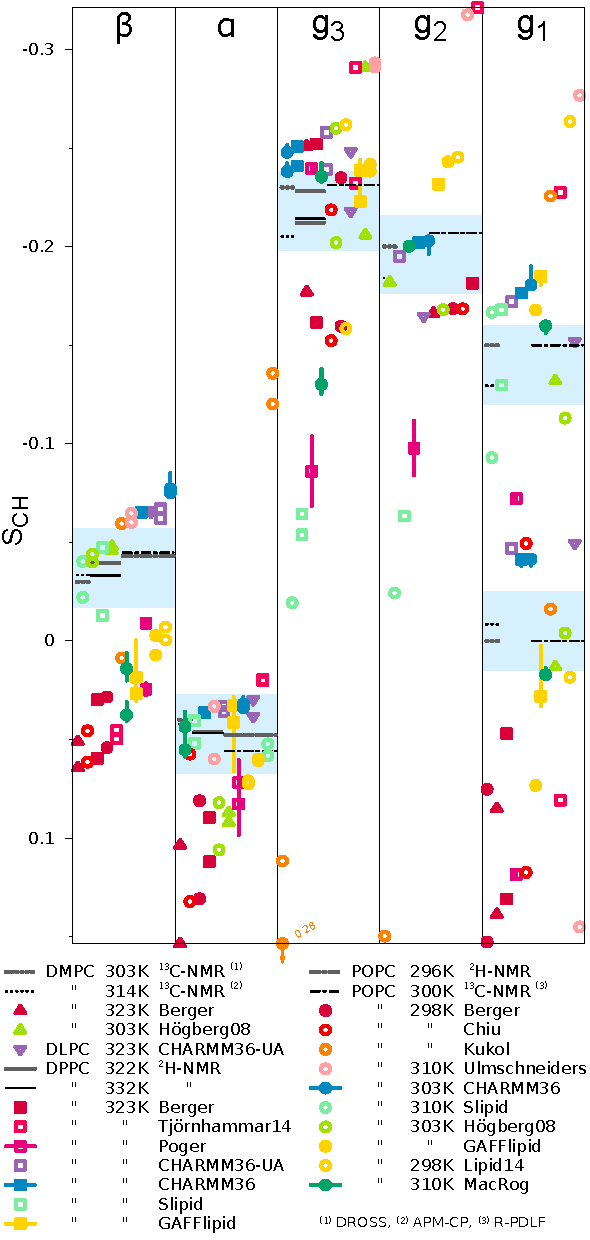
\includegraphics[width=8.6cm]{../DATAreportediINblog/comparisonSorted.pdf}
%\todo{Markus Miettinen suggested that we should consider making one more figure where only experimental data would be shown and that would be discussed in Section~\ref{experiments}. \\
%COMMENT: I do not think that we need such figure anymore since this figure is more clear now.} \\
\newline
\todo{There is also the interactive version by Hubert Santuz now in https://plot.ly/~HubertSantuz/72/lipid-force-field-comparison/
we should figure out which is the most practical way to put that behind permalink once it finalized (Zenodo, figshare or something else?) and then put a citation in the paper.}
  \caption{\label{HGorderparameters}
  Order parameteres from simulations listed in Table~\ref{systems} and experiments for glycerol and choline groups.
The experimental values were taken from the following publications:
 DMPC 303~K from \cite{gross97},
 DMPC 314~K from \cite{dvinskikh05a},
 DPPC 322~K from \cite{gally75},
 DPPC 323~K from \cite{akutsu81},
 POPC 296~K from \cite{bechinger91}, and
 POPC 300~K from \cite{ferreira13}.
  The vertical bars shown for some of the computational values are not error bars, but demonstrate that for 
these systems we had at least two data sets (see Table~\ref{systems});
the ends of the bars mark the extreme values from the sets, and the dot marks their measurement-time-weighted average. 
} 
\end{figure}

In general there is a good agreement between the order parameters measured with different experimental NMR techniques: Almost all the 
reported values are within a variation of $\pm$0.02 (which is also the error estimate given by Gross et al.~\cite{gross97}) 
for all fully hydrated PC bilayer, regardless of the variation in their acyl chain composition and temperature.
Exceptions are the somewhat lower order parameters sometimes reported from measurements using $^1$H-$^{13}$C NMR~\cite{hong95a,hong95b,warschawski05}.
These experiments are not shown in Fig.~\ref{HGorderparameters} as the reported error bars are either relatively large~\cite{hong95a,hong95b}, 
or the spectral resolution is quite low and the numerical lineshape simulations have not been used in the analysis~\cite{warschawski05}.
Due to this end, it is highly likely that these reported lower order parameters are due to lower experimental 
accuracy and therefore we exclude them from our discussion. 
For more details, see \url{http://nmrlipids.blogspot.fi/2014/02/accuracy-of-order-parameter-measurements.html}
\todo{Citation to the blog will be added when available.}
Motivated by the high experimental repeatability, we have highlighted in 
Fig.~\ref{HGorderparameters} the subjective sweet spots (light blue areas), within which we expect the calculated absolute 
values of the order parameters of a well-performing force field to fall.

%In addition to the phosphatidylcholine lipids, similar values of the glycerol backbone order parameters have been measured
%for phophatidylethanolamine (PE) and phopshatidylglycerol (PG) in E. Coli extract~\cite{gally81},
%indicating that the glycerol backbone structure is similar independent of the headgroup chemistry and lipid environment.
%Further, choline order parameters measured from mouse fibroblast L-M cell are similar to the ones in model
%membranes~\cite{scherer87}.

In addition to the numerical values, an important feature of the glycerol backbone is the 
forking (see section~\ref{expORDp}) of the order parameters in g$_1$ and g$_3$ segments, in contrast to the choline segments $\alpha$ and $\beta$. 
The forking in glycerol backbone g$_3$ segment is small ($\approx$ 0.02) 
and some experiments only report the larger value or the average value~\cite{akutsu81,ferreira13}. 
In contrast, forking is significant for the glycerol backbone g$_1$ segment, whose lower order parameter is close to zero and the
larger one has an absolute value of approximately 0.13--0.15. Forking was studied in detail by Gally et al.~\cite{gally81}, who used E. Coli to 
stereospecifically deuterate the different hydrogens attached to the g$_1$ or g$_3$ groups in PE lipids, and measured the order parameters from the lipid 
extract. This experiment gave the lower order parameter when deuterium was in the S position of g$_1$ or R position for g$_3$.
Since the glycerol backbone order parameters are very similar irrespective of the headgroup chemistry (PC,PE and PG) or lipid 
environment~\cite{gally81}, it is reasonable to assume that the stereospecifity measured for the PE lipids
holds also for the PC lipids.

The most detailed experimentally available order parameter information for the glycerol backbone and choline 
segments of POPC bilayer is collected by taking the absolute values from~\cite{ferreira13}, the signs from~\cite{hong95a,hong95b,gross97} 
and the stereospecific labeling from~\cite{gally81}, and shown in Fig.~\ref{HGorderparameters2}.
\begin{figure*}[]
  \centering
  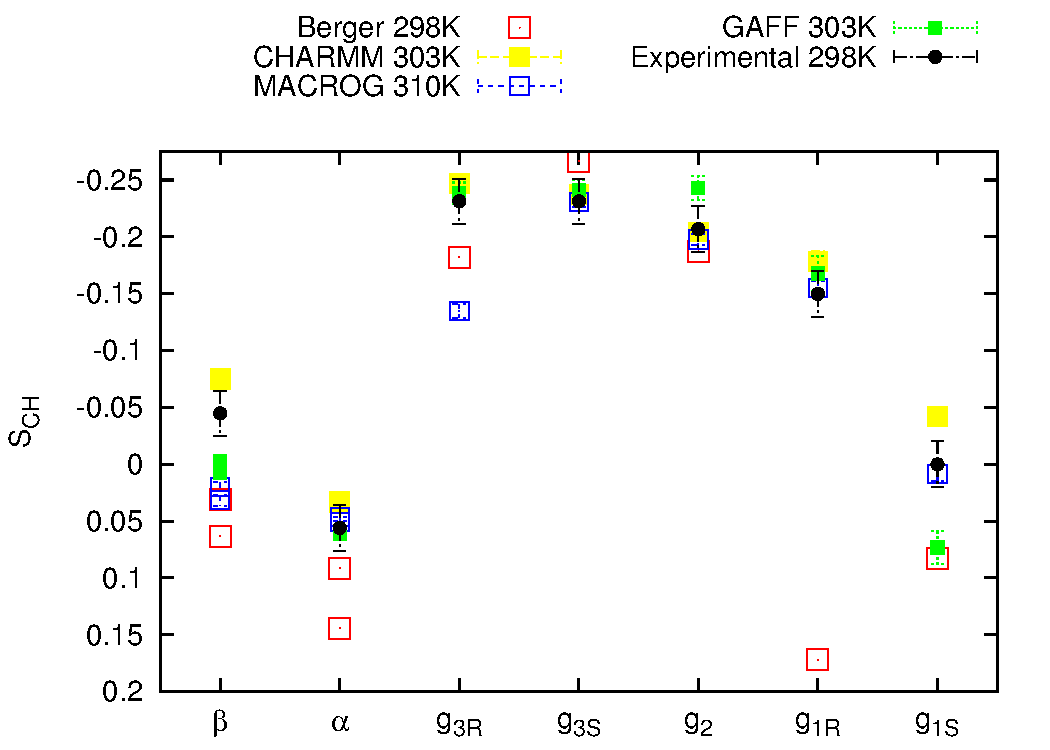
\includegraphics[width=8.6cm]{../Fig/HGorderparameters5.pdf} \\
  \todo{This figure should be updated similar to Fig.~\ref{HGorderparameters}} \\
  \caption{\label{HGorderparameters2}
  Order parameteres from simulations with Berger-POPC-07, CHARMM36, GAFFlipid and MacRog force fields together with experimental values for POPC glycerol and choline groups.
  The magnitudes for experimental order parameters are taken from Ferreira et al.~\cite{ferreira13}, the signs are based on the measurements by Hong et al.~\cite{hong95a,hong95b} 
  and Gross et al.~\cite{gross97}, and the R/S labeling is based in the measurements by Gally et al.~\cite{gally81}.
} 
\end{figure*}

\subsection{Full hydration: Comparison between simulation models and experiments}

The order parameters of the glycerol backbone and headgroup calculated from different force fields for various lipids have been 
previously compared to experiments~\cite{shinoda97,hogberg08,castro08,klauda10,kapla12,dickson12,poger12,ferreira13,chowdhary13,maciejewski14}. 
The general conclusion from these studies seems to be that the CHARMM based~\cite{hogberg08,klauda10}, GAFFlipid~\cite{dickson12} and
MacRog~\cite{maciejewski14} force fields perform better for the glycerol backbone and headgroup structures than the GROMOS based models~\cite{castro08,kapla12,poger12,ferreira13}.
However, none of the studies exploits the full potential of the available experimental data discussed in previous section, i.e. the quantitative accuracy, known signs and stereospecific labeling of
the experimental order parameters.

To get a general idea of the quality of the glycerol backbone and choline headgroup structures in different models, we calculated 
the order parameters for these parts from thirteen different lipid models (Table~\ref{systems}) and 
plotted the results together with experimental values in Fig.~\ref{HGorderparameters}.
Two criteria were used to judge the quality of the model: there must not be significant  {\bf forking} in the $\alpha$ and $\beta$ carbons,
there must be only moderate forking in the g$_3$ carbon and there must be significant forking in the g$_1$ carbon, the {\bf magnitude}
should be preferably inside to the subjective sweet spots determined from experiments (blue shaded regions in Fig.~\ref{HGorderparameters}).
The results for each force field in respect to the above criteria are summarized in Figure~\ref{FullHydrationComparisonTable}.
\begin{figure}[]
  \centering
  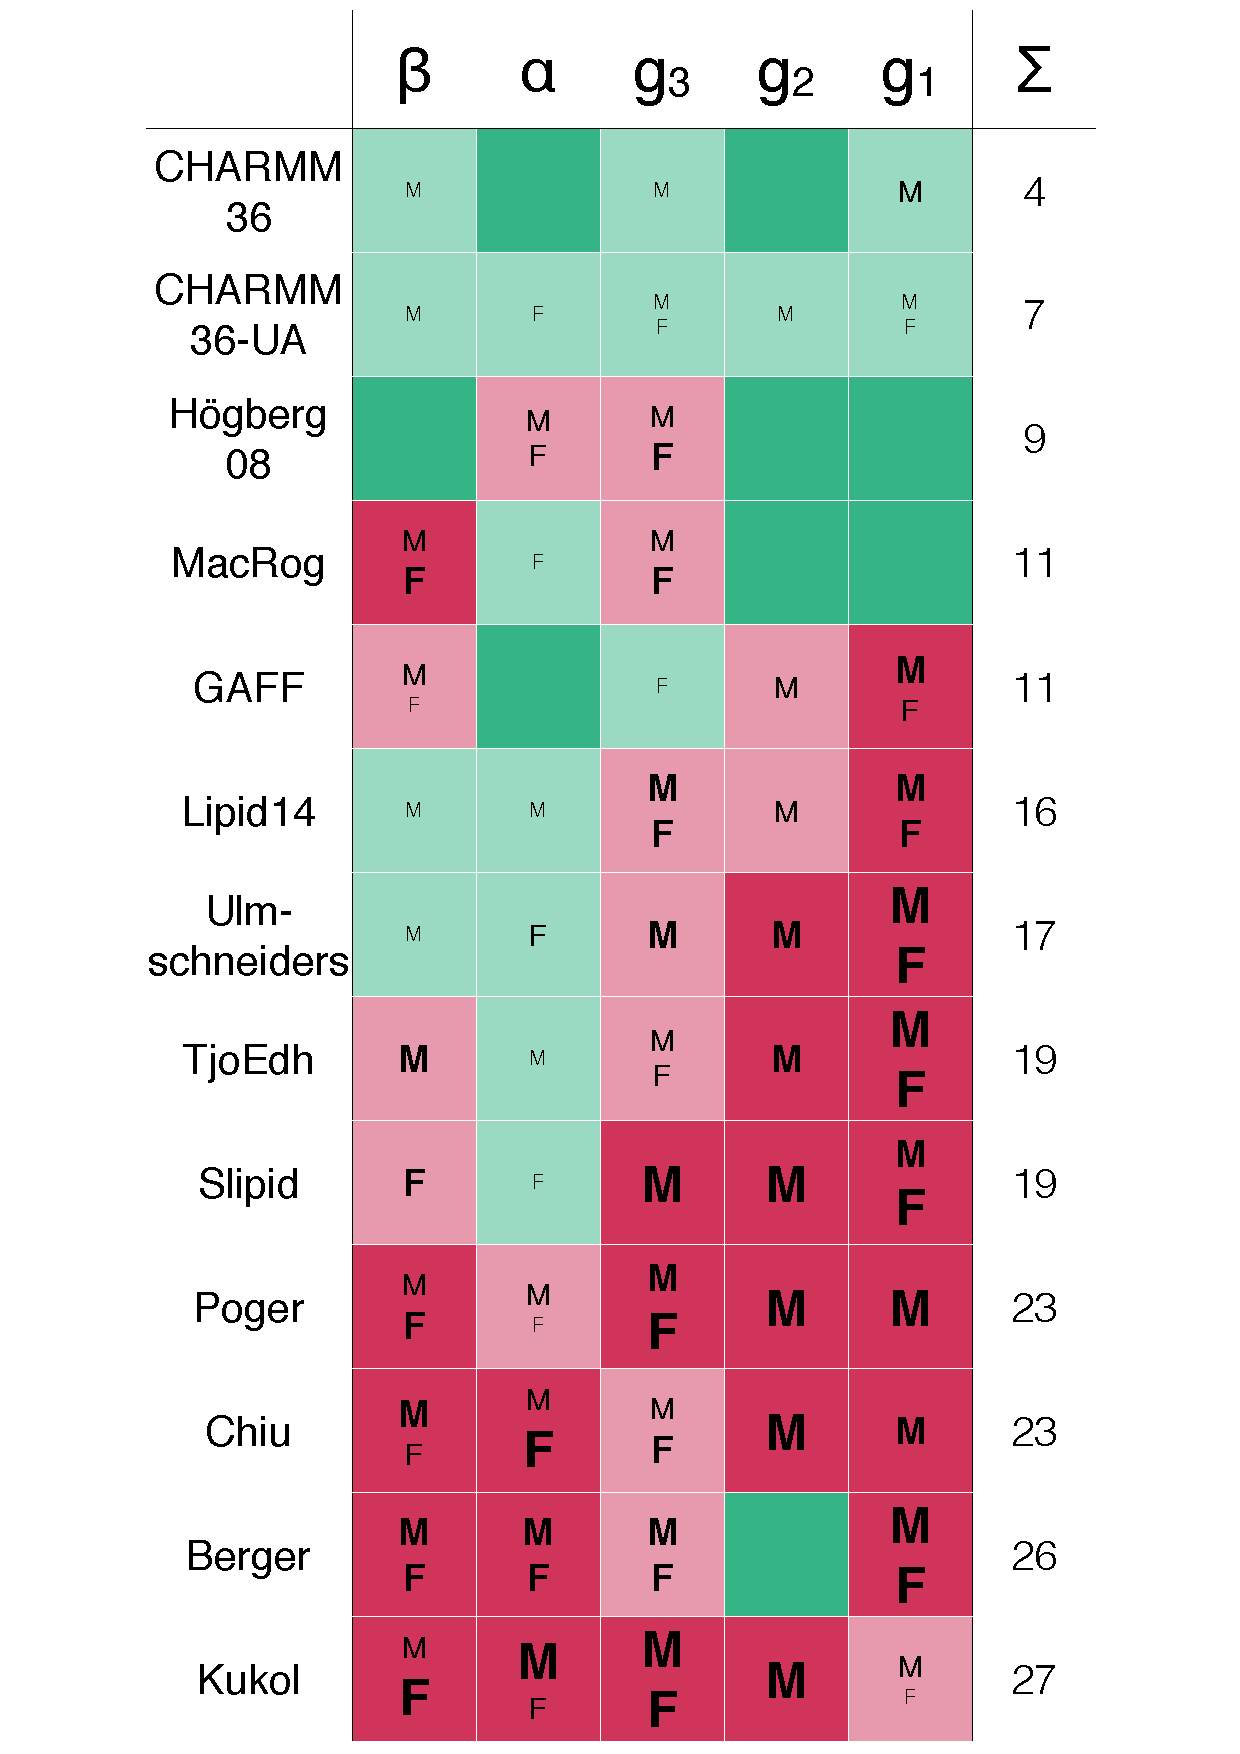
\includegraphics[width=8.6cm]{../DATAreportediINblog/comparisonTable.pdf}
  \newline
  \caption{\label{FullHydrationComparisonTable}
Rough ranking of force fields based on data of Fig.~\ref{HGorderparameters}.
"M" indicates a magnitude problem,
"F" a forking problem.
Letter size shows the level (0-4) of severity;
the $\Sigma$-column shows the sum of these, i.e., the "total severity".
Color scheme:
"within experimental error" (dark green),
"almost within experimental error" (light green),
"clear deviation from experiments" (light red), and
"major deviation from experiments" (dark red).
  } 
\end{figure}

None of the studied force fields fulfils these criteria completely, however CHARMM36 is pretty close. 
This is not surprising since the dihedral potentials in this model are tuned to reproduce these parameters better against experiments~\cite{klauda10}.
The next models in the list are CHARMM36-UA~\cite{henin08,lee14} and H\"ogberg08~\cite{hogberg08} which is also not surprising since
these models are using CHARMM bonded potentials for glycerol backbone and choline. The fourth and the fifth models in the list, MacRog~\cite{maciejewski14} and
GAFFlipid~\cite{dickson12}, have independently determined dihedral potentials. All the models based on Gromos potentials and Slipids perform less well.
In the present work we subject the CHARMM36, MacRog, GAFFlipid and Berger-POPC-07 to a more careful comparison including the sterospecific labeling  
(Fig.~\ref{HGorderparameters2}), and atomistic level structure and responses to the dehydration and cholesterol content in the following sections.
These models are selected for more detailed studies since they are the best representatives of different dihedral potential parametrization techniques 
(CHARMM36, MacRog, GAFFlipid), and the Berger based models are the most used lipid model in the literature.


\subsection{Full hydration: Atomistic resolution structures in different models}

The results in the previous section revealed significant differences of the glycerol backbone and choline headgroup
order parameters between different molecular dynamics simulation models.
However, it is not straightforward to conclude which kind of structural differences (if any)
between the models the results indicate, because the mapping from the order parameters to the 
structure is not unique. In this section we demonstrate that 1) the differences in order parameters
indicate significantly different structural sampling strongly correlating with the dihedral angles of the related bonds,
and that 2) the comparison between experimental and simulated order parameters can be used to exclude
nonrealistic structural samping in molecular dynamics simulations. The demonstration is done for 
the dihedral angles defined by the g$_3$-g$_2$-g$_1$-O(\textit{sn}-1) segments in the glycerol backbone and 
the N-$\beta$-$\alpha$-O segments in the headgroup. These dihedrals were chosen for demonstration, because 
significant differences between the models are observed around these segments in Fig.~\ref{HGorderparameters2}.
We note that performing a similar comparison through all the dihedrals in all the 13 models would probably give highly useful
information on how to improve the accuracy of the models yet this is beyond the scope of the current report. 

The dihedral angle distributions for the  g$_3$-g$_2$-g$_1$-O(\textit{sn}-1) dihedral calculated from different models are
shown in Fig.~\ref{dihDISTS}. The distribution is qualitatively different for the Berger-POPC-07 model, showing a maximum in 
the gauche$^+$-conformation (60$^o$) compared to all the other models showing a maximum in the anti-conformation (180$^o$).
The distributions in all the other models have the same general features, the main difference being that the
fraction of configurations in the gauche$^-$-conformation (-60$^o$) is zero for the MacRog, detectable for the CHARMM36 and
equally large to the gauche$^+$ fraction in GAFFlipid. From the results we conclude that most likely the wrongly sampled
dihedral angle for the g$_2$-g$_1$ bond explains the significant discrepancy to the experimental order parameters
for the g$_1$ segment in the Berger-POPC-07 model (Fig.~\ref{HGorderparameters2}). 
In conclusion, models preferring the anti conformation for this dihedral give more realistic order parameters and
this is in agreement with previous crystal structure and $^1$H NMR studies~\cite{hauser80,hauser81,hauser81b,hauser88,pascher92,marsh06}.
\begin{figure}[]
  \centering
  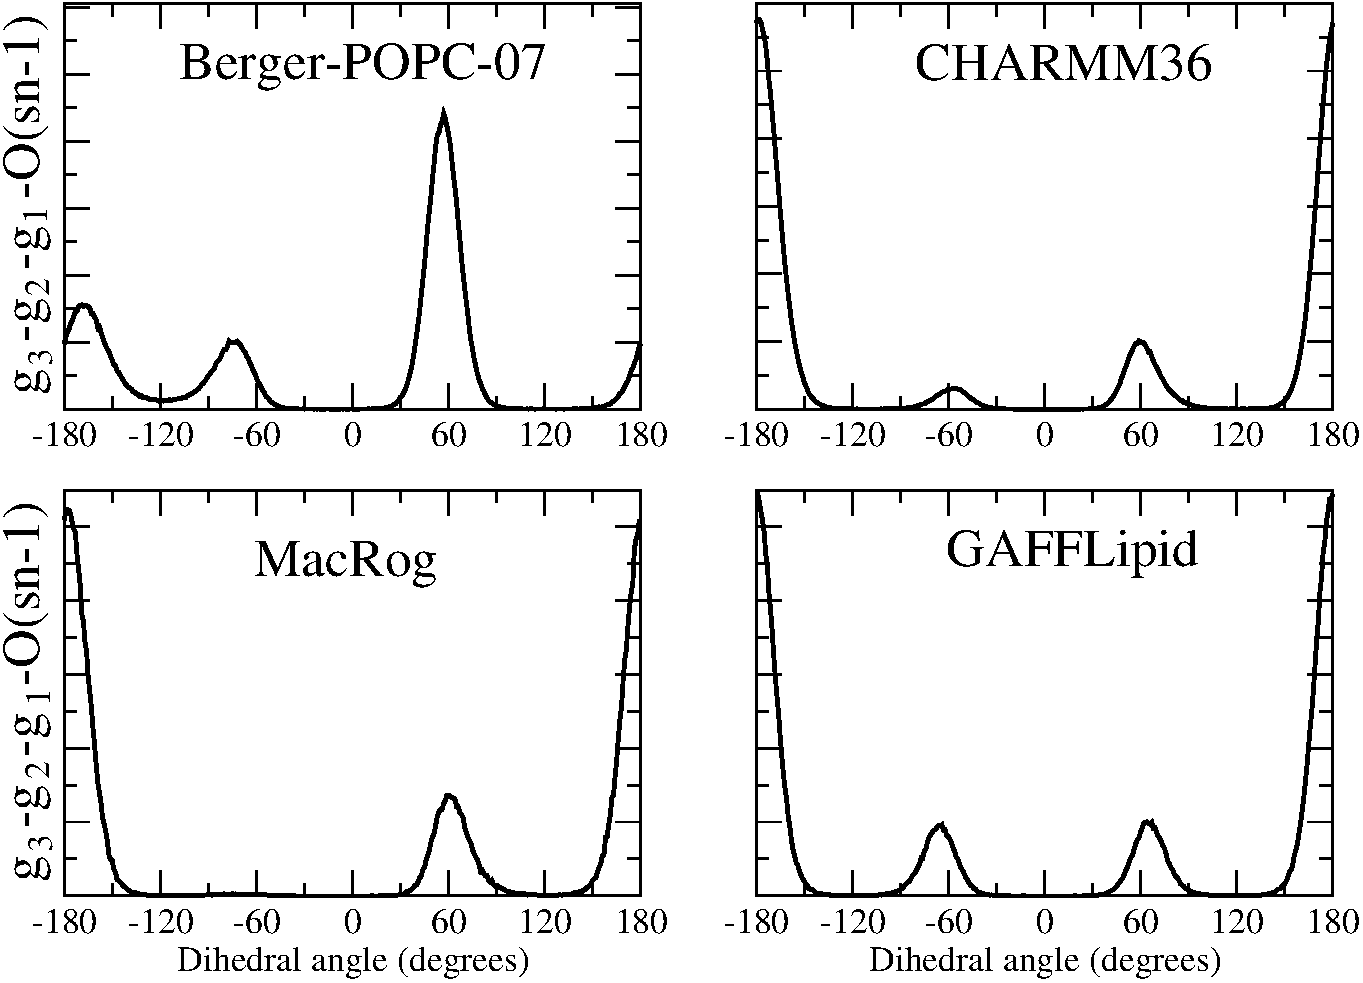
\includegraphics[width=8.6cm]{../Fig/g1-g2_Cdihs2.pdf}
  \caption{\label{dihDISTS}
    Dihedral angle distributions for g$_3$-g$_2$-g$_1$-O(\textit{sn}-1) dihedral from different models (POPC bilayer in full hydration).
      } 
\end{figure}

The dihedral angle distribution for the  N-$\beta$-$\alpha$-O dihedral calculated from the same four models is 
shown in Fig.~\ref{dihDISTS2}. Also for this dihedral there are significant differences in the gauche--anti fractions.
The gauche conformations are dominant in the CHARMM36, in MacRog there are only anti conformations present,
and in the Berger-POPC-07 and GAFFlipid gauche and anti conformations have equal probabilities. 
On the other hand, comparison of $\alpha$ and $\beta$ order parameters in Fig.~\ref{HGorderparameters2}
reveals that for these carbons the CHARMM36 is closest to the experimental results and it is also the only model that has the correct
sign (negative) for the $\beta$ order parameter. This result is again in agreement with previous 
crystal structure, $^1$H NMR and Raman spectroscopy studies~\cite{hauser80,hauser81,hauser81b,akutsu81b} which suggest that
this dihedral is in the gauche conformation in the absence of ions.

%Interestingly, the probability of the gaughe conformations correlates with the order parameter difference between the $\beta$ and $\alpha$ segments:
%the larger the gaughe fraction the larger the order parameter difference. This suggestion together with the results in 
%Fig.~\ref{HGorderparameters2} would indicate that the correct gaughe-trans fraction for N-$\beta$-$\alpha$-O dihedral is 
%larger than in GAFFlipid but smaller than in CHARMM36. This happens to be quite close to the gaughe-trans fraction in
%the Berger model. However, there is significant forking and numerical values are off from the experiments in the Berger
%model suggesting that it has some other inaccuracies.
\begin{figure}[]
  \centering
  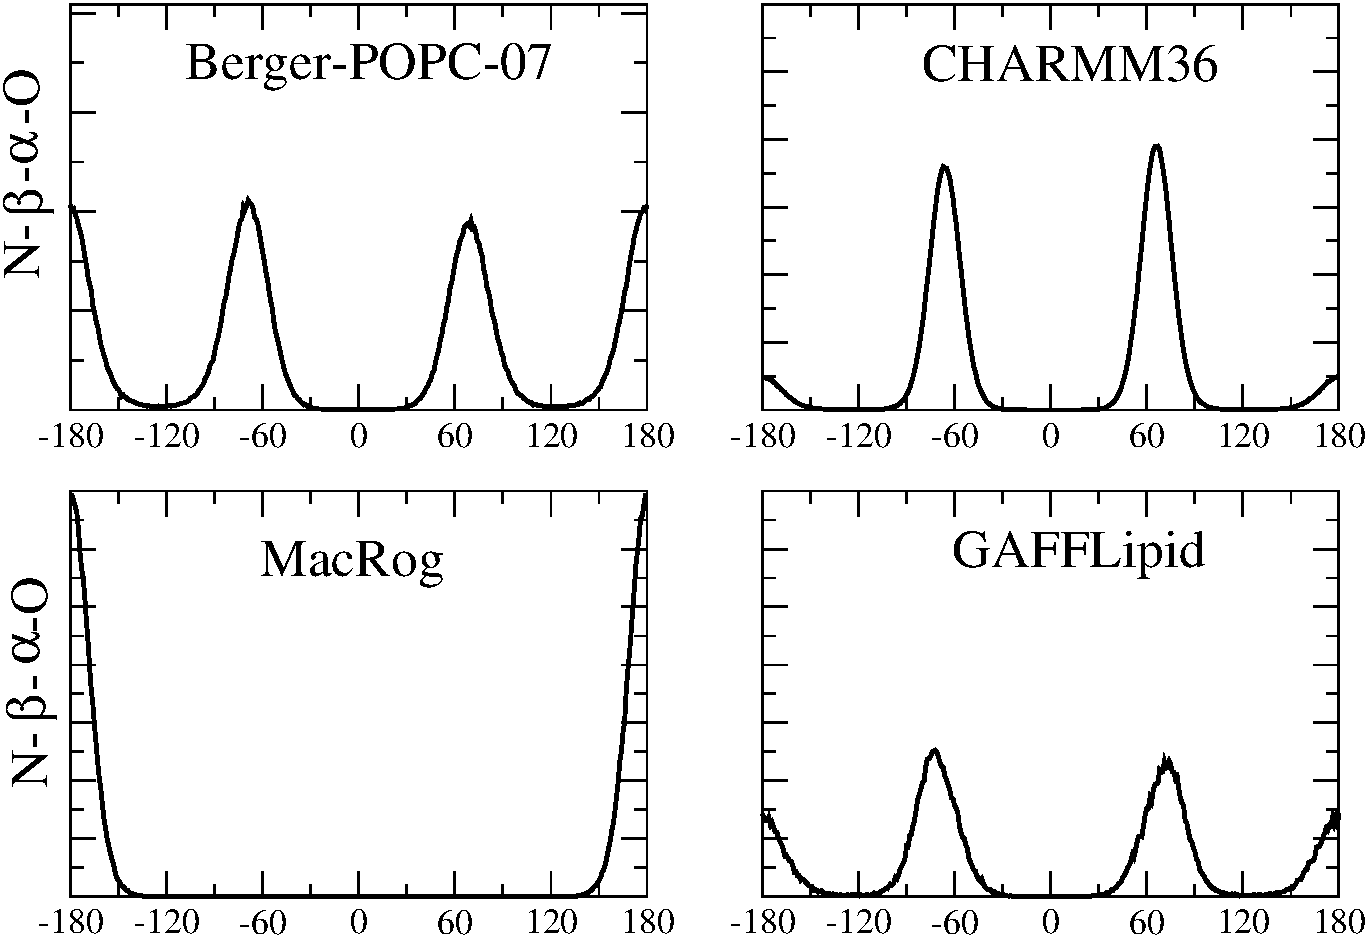
\includegraphics[width=8.6cm]{../Fig/a-bDIHS2.pdf}
  \caption{\label{dihDISTS2}
    Dihedral angle distributions for N-$\beta$-$\alpha$-O dihedral from different models (POPC bilayer in full hydration).
  } 
\end{figure}

The used examples show that the glycerol backbone and headgroup order parameters reflect the atomistic resolution structure
and that the comparison with experiments allows the assessment of the quality of the suggested structure. We were able to pinpoint
specific problems in the structures in different models and suggest potential improvement strategies.
If the improved atomistic
molecular dynamics simulation model reproduced the order parameters and other experimental observables (like chemical shift anisotropy)
with experimental accuracy, it would give an interpretation for the atomistic resolution structure of the glycerol backbone and 
choline~\cite{seelig77b,skarjune79,jacobs80,davis83,akutsu91,hong95b,semchyschyn04}. The research along these lines is left, however,
for future studies.


\subsection{Response to dehydration and cholesterol content}
In addition to pure phosphatidylcholine bilayers at full hydration, the choline headgroup order parameters
have been measured under various different conditions~\cite{gally75,brown77,brown78,akutsu81,altenbach84,scherer89,bechinger91,ulrich94,dvinskikh05b,castro08,kapla12,ferreira13}.
Also the order parameters for the glycerol backbone have been measured with $^1$H-$^{13}$C NMR in dehydrated conditions~\cite{dvinskikh05b}, and as a function 
of anesthetics~\cite{castro08} and glycolipids~\cite{kapla12} for DMPC, and as a function of cholesterol 
concentration for POPC~\cite{ferreira13}. Due to the high resolution in the NMR (especially $^2$H NMR) experiments,
even very small order parameter changes resulting from the varying conditions can be measured (see
\url{http://nmrlipids.blogspot.fi/2014/02/accuracy-of-order-parameter-measurements.html}
for more discussion.)
\todo{Citation to the blog will be added when available.}
However, as already discussed above, it is not simple to deduce 
the structural changes from order parameter changes~\cite{akutsu91,semchyschyn04}. Consequently, comparison of the order parameters
between simulations and experiments in different conditions can be used to assess the quality of the force field 
in different situations, and, if the quality is good, to potentially interpret the structural changes in experiments.
Here we exemplify such comparison for a lipid bilayer under low hydration levels and when varying amounts of cholesterol is included in the bilayer. 
The interaction between ions and a phosphatidylcholine bilayer will be discussed in a separate study~\cite{ionpaper}.


\subsubsection{Phospholipid bilayer with low hydration level}
The experimental order parameters available in the literature~\cite{dvinskikh05b,ulrich94,bechinger91} 
for the glycerol backbone and choline as a function of hydration level are shown in Fig.~\ref{ordPhydr}. 
The independently reported values for choline segments are in good agreement with each other (despite 
slight differences in temperature and acyl chain composition),
showing increase for both segments with decreasing hydration level. It should be noted that only 
absolute values were measured in the original experiments~\cite{dvinskikh05b,ulrich94,bechinger91}, but
we have included the signs measured in separate studies~\cite{hong95a,hong95b,gross97}. 
Consequently, the $\beta$ order parameter with negative sign actually increases with dehydration 
since the absolute value decreases~\cite{dvinskikh05b,ulrich94,bechinger91}.
Slight decrease for the glycerol backbone order parameters were observed with dehydration~\cite{dvinskikh05b}.
\begin{figure}[]
  \centering
  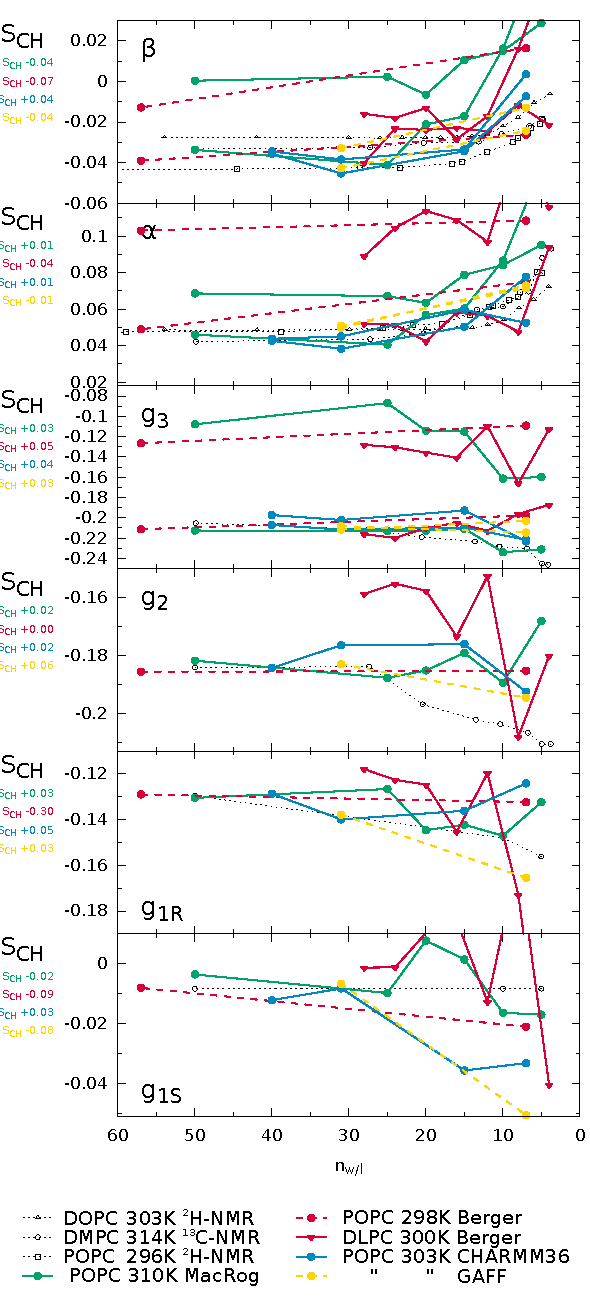
\includegraphics[width=8.6cm]{../DATAreportediINblog/dehydration.pdf} \\
  \todo{DONE} \\
  \caption{\label{ordPhydr}
    The effect of dehydration on glycerol and choline order parameters in experiments.
    The magnitudes of order parameters are measured for DMPC ($^1$H-$^{13}$C NMR) at 314~K~\cite{dvinskikh05b}, 
    for POPC ($^2$H NMR) at 296~K~\cite{bechinger91} and for DOPC ($^2$H NMR) at 303~K~\cite{ulrich94}. 
    The signs are based on the measurements by Hong et al.~\cite{hong95a,hong95b} 
    and Gross et al.~\cite{gross97}.
    Note that to elucidate the relative change as a function of hydration level,
    the simulation results are shifted such that the (smaller) $S_\mathrm{CH}$
    matches (within $\pm$0.01) the experimental value at full hydration;
    the shift magnitudes for each of the force fields are listed ($S_\mathrm{CH}$+shift) in the y-label.
  }
\end{figure}

Lipid bilayer dehydration has been studied also with molecular dynamics simulations~\cite{mashl01,pertsin05,pertsin07,eun09,eun10,schneck12},
typically motivated by the  discussion about the origin of the ``hydration repulsion''~\cite{israelachvili,israelachvili96,sparr11}.
However, the used simulation models are not typically compared to the experimental choline and glycerol backbone
order parameters (except by Mashl et al.~\cite{mashl01}).
In Fig.~\ref{ordPhydr} the glycerol backbone and choline order parameters are shown as a function of hydration level for the CHARMM36, 
MacRog and GAFFlipid models (having the most realistic atomistic resolution structures) together with the Berger based model 
(which is the most used lipid model). 
To elucidate changes the simulation results are shifted to match better with experiments with full hydration.
The magnitude of shifting is written in the y-axis label.
The choline order parameter increase with dehydration is seen in all
models despite of some additional fluctuations. Thus the choline order parameter response to dehydration can be
intepreted to be in qualitative agreement with experiments.
The situation is significantly more complicated for the glycerol backbone segments 
and none of the models can be interpreted to qualitatively agree with experiments
for all the segmets.
\todo{DONE}

The qualitative agreement with experiments in all simulation models for the $\alpha$ and $\beta$ order parameters  
as a function of hydration indicates that the structural response of the choline headgroup to dehydration is somewhat realistic
despite the unrealistic structures at full hydration. 
The most likely explanation is that the choline group
orients more parallel to the membrane plane with dehydration due to restricted interlamellar space. 
Indeed, the P--N (phoshate phosphorus to choline nitrogen) vector angle with membrane normal shows an increase for
all models as a function of dehydration in Fig.~\ref{PNangle}.
However, the amount of increase depends on the model. Especially the DLPC simulations with Berger model
predict significantly stronger P--N vector tilt compared with the other models. The Berger model
has also generally larger P--N vector angles and its choline order parameters are more off from
experiments than other models. Thus the relatively modest tilting with dehydration
predicted by MacRog, CHARMM36 and GAFFlipid is probably more realistic.

It should be also noted that the free energy landscape is not correct in the models which
are not able to reproduce the experimental order parameters. Thus the energetical response
to the dehydration may not be correct even though the order parameter response is qualitatively correct.
This issue may have some influence on the dehydration energetic calculations made with the Berger model~\cite{eun09,schneck12}.
\begin{figure}[]
  \centering
  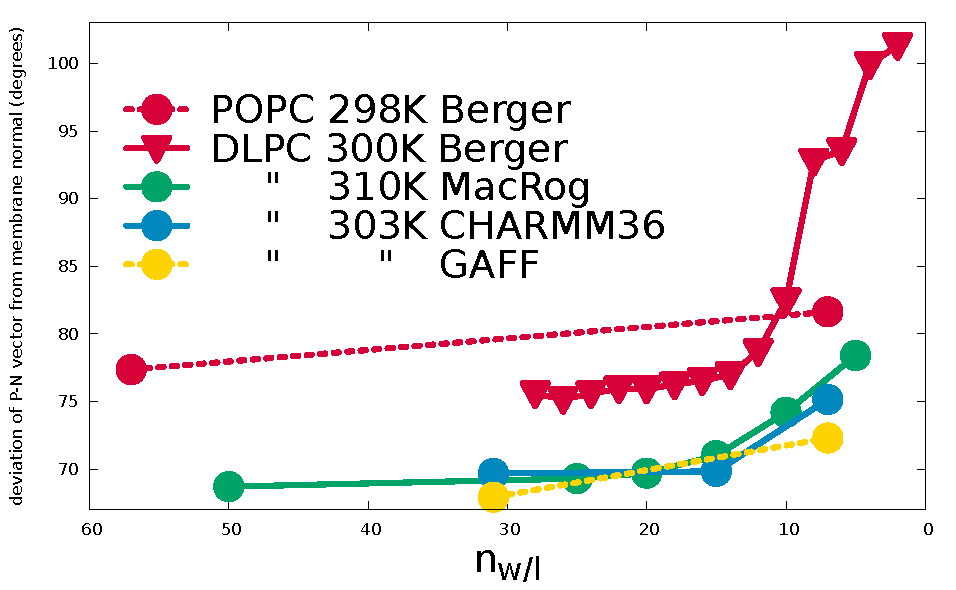
\includegraphics[width=8.6cm]{../Fig/dehydrationPN.pdf}

  \caption{\label{PNangle}
    The angle between membrane normal and P--N vector as function of
    hydration level calculated from different simulations.
  }
\end{figure}

The response of the glycerol backbone to dehydration seems to be more subtle than that of the choline headgroup 
and none of the models reproduced the experimental results with the accuracy allowing
the structural interpretation.
\todo{DONE}


\subsubsection{Cholesterol-containing phospholipid bilayer}
Phospholipid--cholesterol interactions have been widely studied with theoretical~\cite{huang99,zhu07,rog09,alwarawrah12} and
experimental methods~\cite{brown78,marsh10,ferreira13,marsh13}, since cholesterol is abundant in biological membranes.
It has been suggested to be an important player, for example, in domain formation~\cite{simons04,somerharju09}.
It is widely agreed that cholesterol orders lipid acyl tails thus decreasing the area per molecule (condensing effect),
however, the influence of cholesterol on the lipid headgroup and glycerol backbone are sill debated~\cite{huang99,simons04,somerharju09}.
For example, it has been suggested that the surrounding lipids shield cholesterol from interactions with water by 
reorienting their headgroups (``umbrella model'')~\cite{huang99} or that cholesterol acts as a spacer for the headgroups thus increasing 
their entropy and dynamics (``superlattice model'')~\cite{somerharju09}. 
%\todo{It has been suggested that we should use direct quotations from original papers here for clarity.}
Both of these suggestions have been supported
by molecular dynamics simulations~\cite{zhu07,alwarawrah12}, and other simulations suggest specific
interactions between the glycerol backbone and cholesterol~\cite{rog09}. However,
in the above mentioned studies, the glycerol backbone and choline headgroup behaviour
as a function of cholesterol content has not been compared to experiments. 

The choline headgroup and glycerol backbone order parameters for POPC measured by $^1$H-$^{13}$C NMR~\cite{ferreira13} and DPPC choline order parameters 
measured by $^{2}$H NMR~\cite{brown78} are shown in Fig.~\ref{ordPchol} as a function of cholesterol content.
The agreement between different experimental results is again very good, showing only very modest changes in 
the choline order parameters as a function of cholesterol content. It should be noted, however, that very small
changes are measurable with high resolution $^{2}$H NMR experiments
and cholesterol causes a measurable increase in the $\beta$ order parameter and a forking in the $\alpha$ order
parameter~\cite{brown78}. These effects are, however, so small that they are barely visible in the scale used in Fig.~\ref{ordPchol}.
Further, the effects of cholesterol on the glycerol backbone order parameters for POPC from $^1$H-$^{13}$C NMR experiment~\cite{ferreira13} 
are in good agreement with the results for the phosphatidylethanolamine (PE) measured by $^{2}$H NMR~\cite{ghosh82}.
These results further support the idea that the glycerol backbone structural behaviour is independent of the
headgroup composition~\cite{gally81} and that the headgroup stucture is independent of the acyl chain region content unless
charges are present~\cite{scherer87}.
\begin{figure}[]
  \centering
  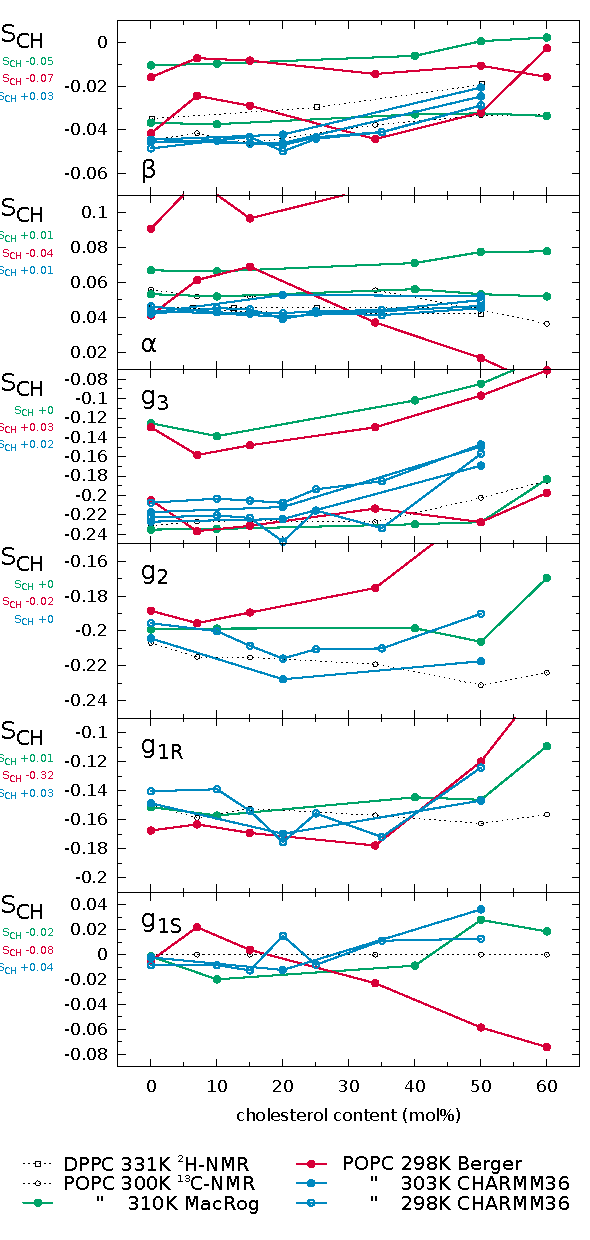
\includegraphics[width=8.6cm]{../DATAreportediINblog/cholesterolization.pdf} \\
  \todo{DONE} \\
  \caption{\label{ordPchol}
    The effect of cholesterol content on the glycerol backbone and choline order parameters in experiments~\cite{brown78,ferreira13} and simulations
    with the Berger-POPC-07/H\"oltje-CHOL-13, CHARMM36 and MacRog force fields. The signs in the experimental values are based on the measurements by Hong et al.~\cite{hong95a,hong95b} 
    and Gross et al.~\cite{gross97}.  Most order parameters from Berger-POPC-07/H\"oltje-CHOL-13 model for g$_1$ are beoynd the y-axis scale.
    Note that to elucidate the relative change as a function of cholesterol content,
    the simulation results are shifted such that the (smaller) $S_\mathrm{CH}$
    matches (within $\pm$0.01) the experimental value without cholesterol;
    the shift magnitudes for each of the force fields are listed ($S_\mathrm{CH}$+shift) in the y-label.
}
\end{figure}

In addition to the experimental data, the previously published simulation results from the Berger-POPC-07/H\"oltje-CHOL-13 model~\cite{ferreira13},
and our results from CHARMM36 and MacRog force fields are shown in Fig.~\ref{ordPchol}. 
To elucidate changes the simulation results are shifted to match better with experiments without cholesterol.
The magnitude of shifting is written in the y-axis label.
As already pointed out previosly, the Berger-POPC-07/H\"oltje-CHOL-13 model
seriously overestimates the effect of cholesterol on the phospholipid glycerol backbone and choline segments~\cite{ferreira13}.
In contrast, the responses of both CHARMM36 and MacRog are in better agreement with experiments. 
%However, CHARMM36 seems to better reproduce the experimentally observed modest changes in the glycerol backbone segments 
%g$_2$ and g$_3$ with high concentrations of cholesterol. 
Thus we have calculated the glycerol backbone dihedral angle distributions
as a function of cholesterol in CHARMM36 (shown in Supplementary material) to resolve the cholesterol induced structural changes. The only detectable change due to the
addition of cholesterol is the small decrease of gauche- and increase of gaughe+ probability of g3-g2-g1-O(\textit{sn}-1) dihedral.


It should be noted that the CHARMM36 force field parameters (dihedral potentials) for the glycerol backbone have been tuned to reproduce the correct order parameters at fully hydrated conditions~\cite{klauda10}. 
This procedure contains a risk of overfitting, which would manifest itself as wrong responses to changing conditions. 
According to our results, this tuning does not seem to lead to overfitting problems in the case of dehydration or lipid--cholesterol mixtures. 


\pagebreak
\section{Conclusions}
The atomistic resolution structures sampled by the glycerol backbone and choline headgroup
in phoshatidylcholine bilayers are not known despite of vast amount of accurate experimental
data. Atomistic resolution molecular dynamics simulation model which reproduced the
experimental data would automatically resolve the structures giving an interpretation of experimental results.
In this work we have collected and reviewed the experimental C--H bond vector order
parameters available in the literature. These experimental parameters are then compared to
different atomistic resolution simulation models for a fully hydrated bilayer, bilayers dehydrated to different extents, and
lipid bilayers containing various amounts of cholesterol. Our results have led to the following conclusions:

- The C--H bond order parameters measured with different NMR techniques are in good agreement
with each others. By combining the experimental results from various sources we concluded
that the order parameters for each C--H bond are known with a quantitative accuracy of $\pm$0.02.

- Comparison of order parameters between experiments and different atomistic resolution models 
together with the structural analysis shows that these parameters can be used
to judge the structural accuracy of the model. Thus the combination of atomistic resolution 
molecular dynamics simulations and NMR experiments can be used to resolve the atomistic resolution
structures of biomolecules in biologically relevant conditions. 
This approach can be extended from lipids also, for example, to membrane proteins.

%None of the tested models (13 different models) produces the order parameters with the experimental
%accuracy for a fully hydrated phoshatidylcholine lipid bilayer. However, the CHARMM36, GAFFlipid and MacRog 
%models are relatively close. The structures of these models together with the most used lipid model (Berger based) 
%were subjected to more careful studies. The results revealed that the current models are not accurate
%enough to resolve the atomistic resolution structures sampled by glycerol backbone and choline headgroup.  
%However, the correlation between dihedral angle distributions and order parameter differences was found, 
%suggesting that careful adjustment of dihedral potentials would potentially lead to the model with a correct
%structure.

- The review of previous experimental results revealed that the 
choline order parameters are increasing when the bilayer is dehydrated. Our simulations suggest that
this can be explained by P--N vector tilting more parallel to the membrane. 
These results strongly supports and complements the idea that the charge induced choline tilting and 
partition can be measured by using the order parameter changes~\cite{ionpaper,scherer89}.

%Independent of the accuracy for a fully hydrated lipid bilayer, all the models reproduced the choline response
%to dehydration. This can be explained by the change in the P--N vector tilting more parallel to the membrane,
%which leads to the increase of order parameters despite of the initial configuration. It should be noted, however,
%that the correct qualitative response does not necessarily indicate correct energetics. 

- Only modest changes of glycerol backbone and choline order parameters are observed experimentally with increasing cholesterol concentration.
When interpreted by using the simulations with the most realistic response to the cholesterol concentration,
this observation can be explained such that the cholesterol induces only minor changes in the g$_3$-g$_2$-g$_1$-O(sn-1)
dihedral in the glycerol backbone.

%- The response of glycerol backbone and choline headgroup to the cholesterol content is described more
%realistically in CHARMM36 and MacRog models than in the Berger based model.

- Besides the main conclusions, we have created the most extensive
publicly available collection of molecular dynamics simulation trajectories of lipid bilayers
into the Zenodo community \url{https://zenodo.org/collection/user-nmrlipids}. 
This collection opens up numerous possiblities for different analyses with
much less effort than previously required.

In general, we conclude that to fully utilize the potential of atomistic resolution classical molecular dynamics simulations
in the structural interpretation of the high resolution NMR data~\cite{ferreira14} for lipid bilayers one has to  
improve the phoshatidylcholine glycerol backbone and choline headgroup parameters.

This work has been done as an open collaboration by using the \url{nmrlipids.blogspot.fi} as an communication
platform. All the scientific contributions have been done through the blog and are publicly
available. \todo{Citation to the blog will be added when available.} 

%This work has been, and continues to be, progressed and discussed through a blog at \url{nmrlipids.blogspot.fi}. 
%Everyone is invited to join the discussion and make contributions through the blog. 
%The manuscript will be eventually submitted to an appropriate scientific journal. 
%Everyone who has contributed to the work through the blog will be offered 
%coauthorship. For more details, see \url{nmrlipids.blogspot.fi}. 


%\listoftodos




%%%%%%%%%%%%%%%%%%%%%%%%%%%%%%%%%%%%%%%%%%%%%%%%%%%%%%%%%%%%%%%%%%%%%
%% The "Acknowledgement" section can be given in all manuscript
%% classes.  This should be given within the "acknowledgement"
%% environment, which will make the correct section or running title.
%%%%%%%%%%%%%%%%%%%%%%%%%%%%%%%%%%%%%%%%%%%%%%%%%%%%%%%%%%%%%%%%%%%%%
\begin{acknowledgement}

\todo{All authors, please add your acknowledgements.}

OHSO acknowledges Tiago Ferreira and Paavo Kinnunen for useful discussions, 
the Emil Aaltonen foundation for financial support, 
Aalto Science -- IT project and CSC -- IT Center for Science for computational resources. 

MSM acknowledges financial support from the Volkswagen Foundation (86110).

WK acknowledges CSC -- IT Centre for Science (Espoo, Finland) is acknowledged for excellent computational resources (project number tty3995).

JM acknowledges CSC -- IT Center for Science for computational resources.


MJ and JT acknowledge and CSC - IT Center for Science for computational resources (project number tty3979).
MJ also acknowledges the Finnish Doctoral Programme in Computational Sciences (FICS) for funding.
JT, MJ, TR and WK acknowledge the funding from the Academy of Finland (Centre of Excellence program) 
and the European Research Council (Advanced Grant project CROWDED-PRO-LIPIDS).


CL and AB acknowledges financial support from the French National Research Agency
(ANR: “Biolubrication by phospholipid membranes” Bioub2012) and
computing time allocation from P{\^o}le Scientifique de Mod{\'e}lisation Num{\'e}rique from the ENS Lyon (PSMN),
and Centre Informatique National de l'Enseignement Sup{\'e}rieur (CINES, Montpelier, France)
(Project c2015096850).

HS acknowleges Catherine Etchebest and St\'ephane T\'eletch\'ea for useful discussions and continued support, the HPC resources granted from GENCI-CINES (Grant 2014-c2014077209) and computer facilities provided by R\'egion Ile de France and INTS (SESAME 2009 project).

Fernando Favela acknowledges CONACYT and DGAPA UNAM IG100513
for financial support, Cluster H\'ibrido de Superc\'omputo Xiuhcoatl - CINVESTAV and Miztli - UNAM for computational resources. 

\end{acknowledgement}

%%%%%%%%%%%%%%%%%%%%%%%%%%%%%%%%%%%%%%%%%%%%%%%%%%%%%%%%%%%%%%%%%%%%%
%% The same is true for Supporting Information, which should use the
%% suppinfo environment.
%%%%%%%%%%%%%%%%%%%%%%%%%%%%%%%%%%%%%%%%%%%%%%%%%%%%%%%%%%%%%%%%%%%%%
\begin{suppinfo}

Simulation details, one figure and author contributions.

%This will usually read something like: ``Experimental procedures and
%characterization data for all new compounds. The class will
%automatically add a sentence pointing to the information on-line:

\end{suppinfo}

%%%%%%%%%%%%%%%%%%%%%%%%%%%%%%%%%%%%%%%%%%%%%%%%%%%%%%%%%%%%%%%%%%%%%
%% The appropriate \bibliography command should be placed here.
%% Notice that the class file automatically sets \bibliographystyle
%% and also names the section correctly.
%%%%%%%%%%%%%%%%%%%%%%%%%%%%%%%%%%%%%%%%%%%%%%%%%%%%%%%%%%%%%%%%%%%%%


\newpage
\begin{center}
{\bf SUPPLEMENTARY INFORMATION}
\end{center}
\subsection{Simulation details} 
\subsubsection{Berger based models}
For the Berger based models we use here the following naming convention: 
Berger - \{{\it molecule name}\} - \{{\it year when model published first time}\} \{{\it citation}\}.
The reason is that there are several different molecular topologies which are using the non-bonded parameters originally
developed by Berger et al.~\cite{berger97}. Thus the common factor in the Berger based models are the non-bonded parameters,
while the molecule specific parameters might somewhat vary. However, the majority of the molecular level topologies are 
relying (especially for the glycerol backbone and headgroup) on the parameters originally introduced by Marrink et al.~\cite{marrink98}.
This is the case for all the Berger based simulations discussed in this work.

POPC simulations at full hydration at 298~K and simulations studying the effect of cholesterol are the same as in previous publications~\cite{ferreira13,ferreira15}.
In these simulation the POPC parameters introduced by Ollila et al~\cite{ollila07a} are used, which are using the non-bonded parameters of Berger~\cite{berger97}
and a molecular topology from Tieleman et al.~\cite{tieleman99} with improved double bond dihedrals by Bachar et al.~\cite{bachar04}. 
Thus they are called Berger-POPC-07~\cite{ollila07a}. The cholesterol model is based on the parameters by H\"oltje et al.~\cite{holtje01} with the
exception that the atom types were changed from CH2/CH3 to LP2/LP3 to avoid overcondensation of the bilayer as suggested in ref.~\cite{tieleman06}.
Since this modification was introduced by Ferreira et al.~\cite{ferreira13}, we call the used cholesterol model as H\"oltje-CHOL-13~\cite{ferreira13}.

For the POPC at 323~K and POPC in low hydration the same force field parameters are used.
For DPPC the implementation of Berger parameters~\cite{berger97} by Peter Tieleman et al. are used~\cite{marrink98}.
For all of these simulations a timestep of 2~fs was used with a leapfrog integrator. Covalent bond lengths were constrained with the LINCS algorithm~\cite{hess97,hess07}. 
Coordinates were written every 10~ps. PME~\cite{darden93,essman95} with real space cut-off of 1.0~nm was used 
for electrostatics. Plain cut-off was used for the Lennard-Jones interactions with a 1.0~nm cut-off.
The neighbor lists with cut-off of 1.0~nm were updated every 5 steps. Temperature was coupled separately
for lipids and water to 298~K using the velocity-rescale method~\cite{bussi07} with coupling constant 0.1~ps.
Pressure was semi-isotropically coupled to the atmospheric pressure with the Berendsen method~\cite{berendsen84}.

\subsubsection{CHARMM36}

{\it DPPC}
\todo{Markus Miettinen, please describe how you made the files.}

Timestep of 1~fs was used with the leapfrog integrator. Covalent bonds with hydrogens were constrained with LINCS algorithm~\cite{hess97,hess07}. 
Coordinates were written every 5~ps. PME~\cite{darden93,essman95} with real space cut-off of 1.4~nm was used 
for electrostatics. Lennard-Jones interactions were switched to zero between 0.8~nm and 1.2~nm.
The neighbour lists with a cut-off of 1.4~nm were updated every 5 steps. Temperature was coupled separately
for lipids and water to 303~K using the velocity-rescale method~\cite{bussi07} with coupling constant of 0.2~ps.
Pressure was semi-isotropically coupled to the atmospheric pressure with the Berendsen method~\cite{berendsen84}.

{\it POPC}
The starting structures for the pure POPC and DOPC simulations was taken from the Slipids~\cite{jambeck12b} website (http://people.su.se/$\sim$jjm/Stockholm\_Lipids/Downloads.html).
The starting structures for mixed POPC/Cholesterol simulations were constructed with the CHARMM-GUI website~\cite{jo08}. 
They contained 100 POPC/24 cholesterol molecules and 80 POPC/80 cholesterol molecules for
the simulations of 20\% cholesterol and 50\% cholesterol respectively. The TIP3P water model~\cite{jorgensen83} was used to
solvate the system.
The publicly available CHARMM36 forcefield parameters (\url{http://www.gromacs.org/@api/deki/files/184/=charmm36.ff\\\_4.5.4\_ref.tgz}) 
by Piggot et al. \cite{piggot12} were used. Cholesterol parameters came
from Lim et al. \cite{lim12} and were converted into GROMACS format with the PyTopol tool~\cite{salari15}.  
Single point energy calculation was done to assess the conversion. 
%(At the time I've made the simulations, the charmm36 ff for cholesterol in gromacs format was not available at
%http://mackerell.umaryland.edu/charmm_ff.shtml#gromacs).
Simulations were performed for 200~ns and the last 100~ns was used for the calculations. Timestep of 2~fs was
used with leapfrog integrator. All bond lengths were constrained with LINCS~\cite{hess97,hess07}. Temperature was maintened at
303~K with the velocity-rescale method~\cite{bussi07} and a time constant of 0.2~ps. Pressure was maintained semiisotropically
at 1~bar using the Parrinello--Rahman algorithm~\cite{parrinello81} with a time constant of 1.0~ps. The neighbour list with a cut-off of 1.2~nm
was updated every 10 steps. Lennard-Jones interactions were switched to zero
between 0.8~nm and 1.2~nm. PME~\cite{darden93,essman95} with real space cut-off of 1.2~nm was used for electrostatics.


\subsubsection{MacRog}
The lipid force field parameters were obtained from the developers and they correspond to the published DPPC parameters~\cite{maciejewski14} with the inclusion of the 
double bond parameters~\cite{kulig15}. 
%This inclusion of unsaturated lipid tails will be published in the near future. 
%\todo{You have recent paper where you use POPC/chol simulations with this model: Kulig et al. BBA 1848 (2015) 422-432 http://dx.doi.org/10.1016/j.bbamem.2014.10.032.
%would this be a correct refence here?}
A bilayer with 288 POPC lipids was hydrated with 12600 TIP3P water~\cite{jorgensen83} molecules ($\sim$44/lipid) and simulated for 100~ns with a time step of 2~fs. Data was saved 
every 10~ps and the first 20~ns of the trajectory was discarded from the analysis. 
All bond lengths were constrained with LINCS~\cite{hess97,hess07}. The temperatures of the lipids and the solvent were separately coupled to the Nos\'{e}--Hoover thermostat~\cite{nose84,hoover85} 
with a target temperature of 310~K and a time constant of 0.4~ps. Semi-isotropical pressure coupling to 1~bar was obtained with the Parrinello--Rahman 
barostat~\cite{parrinello81} with a time constant of 1~ps. PME~\cite{darden93,essman95} was employed to calculate the long-range electrostatic interactions. Lennard-Jones interactions were cut off 
at 1~nm and the dispersion correction was applied to both energy and pressure. A neighbour list with a radius of 1~nm was updated every step. 

Identical parameters were employed for both full hydration and for the dehydration simulations. The dehydration simulations were also run for 100~ns 
with data saved every 10~ps.

The initial structures for the simulations with 10, 40, 50 and 60 mol\% of cholesterol were obtained by replacing 14, 56, 64 or 72 POPC molecules 
with cholesterol molecules in the initial structure containing 128 POPC molecules. These systems were simulated for 400 ns and the first 200 ns was 
discarded from analysis. Data was saved every 100 ps.



\subsubsection{GAFFLipid}
The initial structure in Lipidbook \cite{domanski10} had different glycerol backbone isomers in different leaflets. 
To generate the initial structure we took the structure delivered by Slipids developers~\cite{jambeck12b}. Also this structure
had one lipid with different glycerol backbone isomer. This lipid and one lipid from opposite leaflet were removed
after the system was equilibrated.

The force field parameters were generated using files obtained from the Lipidbook website (\url{http://lipidbook.bioch.ox.ac.uk/package/show/id/150.html})~\cite{domanski10}. 
The conversion to GROMACS compatible formats was performed using the acpype tool~\cite{silva12}. The accuracy of the conversion was checked by calculating 
the total energy of a single POPC lipid molecule using the sander program which is part of the AmberTools14 package~\cite{ferrer13} and version 4.6.5 of GROMACS. 
A difference of 0.002 kcal/mol was obtained between the two programs.

Timestep of 2~fs was used in Langevin dynamics with zero friction term and collision frequency of 1.0~ps$^{-1}$. 
Covalent bonds with hydrogens were constrained with the LINCS algorithm~\cite{hess97,hess07}.
Coordinates were written every 10~ps. PME~\cite{darden93,essman95} with a real space cut-off at 1.0~nm was used 
for electrostatics. Plain cut-off with 1~nm was used for Lennard-Jones interactions. 
The neighbour lists with a cut-off of 1.0~nm were updated every 5 steps. 
Pressure was semi-isotropically coupled to a pressure of 1~bar with the Berendsen method~\cite{berendsen84}.

It should be noted that the area per molecule with these settings for the GAFFlipid model was 61.6~\AA$^2$,
while the original publication reported 63.9~\AA$^2$~\cite{dickson12}. However, the same parameters and Amber to Gromacs
conversion reproduced the area per molecule from original publication for the lipid14 model (see next section).

\subsubsection{Lipid14}
The initial structure was taken directly from the Lipidbook~\cite{domanski10}.
The Amber compatible force field parameters were generated using the tleap program which is integrated in the AmberTools14 package~\cite{ferrer13}. 
A workflow similar to the one used previously for the conversion and validation of the GAFFLipid parameters was followed here. 
As before, a negligible energy difference of 0.003 kcal/mol was obtained between the two programs.

Timestep of 2~fs was used in Langevin dynamics with zero friction term and collision frequency of 1.0~ps$^{-1}$. 
Covalent bonds with hydrogens were constrained with LINCS algorithm~\cite{hess97,hess07}.
Coordinates were written every 10~ps. PME~\cite{darden93,essman95} with real space cut-off of 1.0~nm was used 
for electrostatics. Plain cut-off with 1~nm was used for Lennard-Jones interactions. Dispersion correction
was applied for both energy and pressure. The neighbor lists with a cut-off of 1.0~nm were updated every 5 steps. 
Pressure was semi-isotropically coupled to a pressure of 1~bar with the Berendsen method~\cite{berendsen84}.

The area per molecule with these settings was 65.4~\AA$^2$ which is in agreement with the value reported in the original publication 65.6$\pm$0.5~\AA$^2$~\cite{dickson14}.

\subsubsection{Poger et al.}
The Poger lipids are derived from GROMOS G53A6~\cite{poger10} and were initially coined 53A6-L (L for lipids). They are now part of GROMOS G54A7~\cite{poger12} 
and parametrized to work with the SPC water model~\cite{berendsen81}. The initial hydrated bilayer structure of 128 DPPC and 5841 water molecules as well as force field parameters were downloaded 
from David Poger's web site (\url{http://compbio.chemistry.uq.edu.au/~david/}) on April 2012. 
We noticed that the same files downloaded in October 2013 appear to lack two dihedral angles in the choline headgroup (only one dihedral of type gd\_29 allowing 
the rotation of the 3 choline methyls) compared to the April 2012 version (3 dihedrals of type gd\_29 for the 3 choline methyls). This should not affect the 
bilayer structure and only change the kinetics of the choline methyls rotation. However the October 2013 version has not been tested in this study.

MD Simulations (two repetitions with independent initial velocities) were run for 100~ns using a 2~fs time step and the analysis 
was performed on the last 50~ns. Coordinates were saved every 50~ps for analysis. All bond lengths were constrained with the LINCS algorithm~\cite{hess97,hess07}. Temperature was kept 
at 323~K employing the velocity-rescale~\cite{bussi07} thermostat with a time constant of 0.1~ps (DPPC and water coupled separetly). Pressure was maintained semi-isotropically at 1~bar using 
the Parrinello--Rahman barostat~\cite{parrinello81} using a 4~ps time constant and a compressibility of 4.5e-5~bar$^{-1}$. For non-bonded interactions, two conditions were tested:
i) A 0.8--1.4 nm twin-range cut-off with the neighbor list updated every 5 steps for both electrostatics and Lennard-Jones (LJ) interactions 
(simulation files available at~\cite{pogerFILESrf1,pogerFILESrf2}). For the former the generalized reaction 
field (RF) with a dielectric permittivity of 62 was used beyond the 1.4~nm cut-off~\cite{tironi95}. This is the original setup that Poger et al.~\cite{poger10} used.
ii) PME~\cite{darden93,essman95} electrostatics with a real space cut-off of 1.0~nm, a Fourier spacing of 0.12~nm and an interpolation order of 4, LJ interactions computed with a 1.0--1.4~nm twin-range cut-off,
neighbor list updated every 5 steps (simulation files available at~\cite{pogerFILESpme1,pogerFILESpme2}). 
Note that Poger and Mark tested the effect of PME vs RF in ref.~\cite{poger12}, but used a 1.0~nm cut-off with PME and 1.4~nm with RF for LJ
interactions. Since 0.8--1.4~nm twin-range cut-off for LJ interations is used in the parametrization of GROMOS force field, we decided to use that
also in the simulations with PME.

Since Poger lipids come from the GROMOS force field, it is important to note that GROMOS uses the RF scheme for computing electrostatics (this is the method used for the 
force field parameterization). Using setup i) based on RF, we were able to reproduce the results (i.e. area per lipid value of 0.63~nm$^2$) from the original work only with 
GROMACS versions 4.0.X and earlier (the original authors~\cite{poger10} used GROMACS version 3.3.3). When switching to versions 4.5.X and above, the area per lipid dropped to below 0.58~nm$^2$. 
The GROMACS developers were contacted and a redmine issue opened (\url{http://redmine.gromacs.org/issues/1400}). The difference comes from the new Trotter decomposition 
introduced in versions 4.5.X. A fix has been introduced in version 4.6.6 that allows a recovery of an area per lipid value of 0.615~nm$^2$. The results in terms of area per lipid using the different 
GROMACS versions are available at~\cite{pogerFILESrf2}.
Thus we decided to use only the PME setup ii) for computing the order parameter since it gives stable results regardless of the GROMACS version. We obtained an area per 
lipid of 0.615~nm$^2$, below 0.648 nm$^2$ found by the original authors with their PME setup (see~\cite{poger12}). We explained that by the fact that we used 
a 1.4~nm for the LJ cut-off whereas a value of 1.0~nm was used in the original publication. 

\subsubsection{Slipids}
Initial coordinates for a hydrated DPPC (at 323~K) and POPC (at 310~K) bilayers (30 and 40 waters/lipid, respectively) were taken directly from the 
Slipids home page \url{http://people.su.se/\~jjm/Stockholm\_Lipids/Downloads.html}.  The Slipids force field~\cite{jambeck12,jambeck12b} was used for the the all atom descriptions of DPPC and POPC, and
water was described with the TIP3P water model~\cite{jorgensen83}. Simulations were performed within the NPT ensemble using the GROMACS 4.6.X simulation
package~\cite{hess08}. The Nos\'{e}--Hoover thermostat~\cite{nose84,hoover85} was used with reference temperatures of
323~K (DPPC) and 310~K (POPC) and a relaxation time constant of 0.5~ps. Water and lipids were coupled separately to
the heat bath. Pressure was kept constant at 1.013~bar using a semi--isotropic Parrinello--Rahman
barostat~\cite{parrinello81} with a time constant of 10.0~ps. Equations of motion were
integrated with the leapfrog algorithm using a timestep of 2~fs. Long range
electrostatic interactions were calculated using the PME method~\cite{darden93,essman95}, with a fourth order
smoothing spline. A real space cut-off of 1.0~nm was employed with grid spacing of 0.12~nm in the reciprocal space.
Lennard-Jones potentials were cut off at 1.4~nm, with a dispersion correction applied to both energy and pressure. All covalent bonds in lipids were constrained using the LINCS algorithm~\cite{hess97}, 
whereas water molecules were constrained using SETTLE~\cite{miyamoto92}. Twin-range cutoffs,
1.0~nm and 1.6~nm, were used for the neighbor lists with the longrange neighbor list updated every
10 steps. This simulation protocol corresponds to the protocol used in Ref~\cite{jambeck13}. 

\subsubsection{Kukol}
A bilayer patch with 512 POPC lipids was constructed and hydrated with $\sim$40 SPC water molecules per lipid. 
The force field parameters were obtained from Lipidbook \cite{domanski10}.
This bilayer was simulated with a 2~fs time step for a total of 50~ns and coordinates were saved every 100~ps. 
All bonds were constrained with LINCS~\cite{hess97,hess07}. PME~\cite{darden93,essman95} was employed for the long-range electrostatics. Lennard-Jones interactions 
were cut off at 1.4~nm. A neighbour list with a radius of 0.8~nm was updated every 5~steps. The constant temperature of 298~K 
was maintained with the Berendsen thermostat \cite{berendsen84} with a time constant of 0.1~ps. The Berendsen barostat \cite{berendsen84} 
was employed for semi-isotropical pressure coupling at 1~bar.

\subsubsection{Chiu et al.}
The force field parameters and the initial configuration were available through the Lipidbook~\cite{domanski10}.
Timestep of 2~fs was used with leapfrog integrator. Covalent bond lengths were constrained with LINCS algorithm~\cite{hess97,hess07}. 
Coordinates were written every 10~ps. PME~\cite{darden93,essman95} with real space cut-off of 1.0~nm was used 
for electrostatics. Twin range cut-off was used for the Lennard-Jones interactions with short and long cut-offs of 1.0~nm and 1.6~nm, respectively.
The neighbour lists with a cut-off of 1.0~nm were updated every 5 steps. Temperature was coupled separately
for lipids and water to 298~K with the velocity-rescale method~\cite{bussi07} with a coupling constant 0.2~ps.
Pressure was semi-isotropically coupled to the atmospheric pressure with the Parrinello--Rahman method~\cite{parrinello81}.

\subsubsection{Ulmschneider}
The initial structure containing 128 POPC molecules with 3328 TIP3P water~\cite{jorgensen83} molecules (26 per lipid) was downloaded from Lipidbook \cite{domanski10} 
together with the topologies. This bilayer was simulated for 100~ns with a time step of 2~fs and the data was saved every 10~ps. The bonds involving hydrogen atoms were 
constrained with LINCS~\cite{hess97,hess07}. The temperature was kept at 298~K with the Berendsen thermostat~\cite{berendsen84}. The pressure was semi-isotropically coupled to the Berendsen 
barostat~\cite{berendsen84} with a time constant of 1~ps and a target pressure of 1~bar. PME~\cite{darden93,essman95} was employed for long range electrostatics and a cut-off of 1~ns was employed for 
the Lennard-Jones interactions. A neighbour list with a radius of 1~nm was updated every 10~steps. 

Additionally, the simulations were repeated with the dispersion correction applied to pressure and temperature. Even though the area per lipid decrease
d slightly, the headgroup order parameters were only slightly affected.

\subsubsection{Tj\"ornhammar et al.}
The gel phase DPPC bilayer structure delivered by Tj\"ornhammar  and Edholm~\cite{tjornhammar14} was ran for 5~ns at 343~K in order to destroy the 
ordered gel configuration. This was followed by a 200~ns simulation at 323~K, i.e. in the fluid phase. The last 100~ns of this simulation was used for analysis. 
The same mdp file as in the Supplementary Information section of the original paper ~\cite{tjornhammar14} was used except for the simulation temperature.

\subsubsection{CHARMM36-UA}
A hydrated bilayer consisting of 128 DLPC lipids and 3840 water molecules is modeled by the force field of Lee and co-workers~\cite{lee14}.
This force field is a combination of the all-atom CHARMM36 force-field~\cite{klauda10} and the united-atom Berger model~\cite{berger97}. 
The non-bonded interactions are calculated using an atom-based switching function with short and long cut-offs of 0.8 and 1.2~nm~\cite{lee14}. 
Long range electrostatic interactions are implemented using the particle-particle particle-mesh solver with a relative accuracy of $10^{-4}$. The system 
is first equilibrated for 30~ns in the NP$\gamma$T ensemble (Nos\'{e}--Hoover~\cite{nose84,hoover85} style thermostat and barostat with anisotropic pressure coupling) 
at 323~K and 1~bar with timestep of 1~fs. The following 20~ns of dynamics are taken for calculation of configurational averages. 
Simulations were carried out by using the LAMMPS package~\cite{plimpton95}. %( http://doi.org/10.1006/jcph.1995.1039 )., the input files are available ( http://dx.doi.org/10.5281/zenodo.13821 ).

\subsection{Dihedral angle distributions as a function of cholesterol in CHARMM36}
\begin{figure*}[]
  \centering
  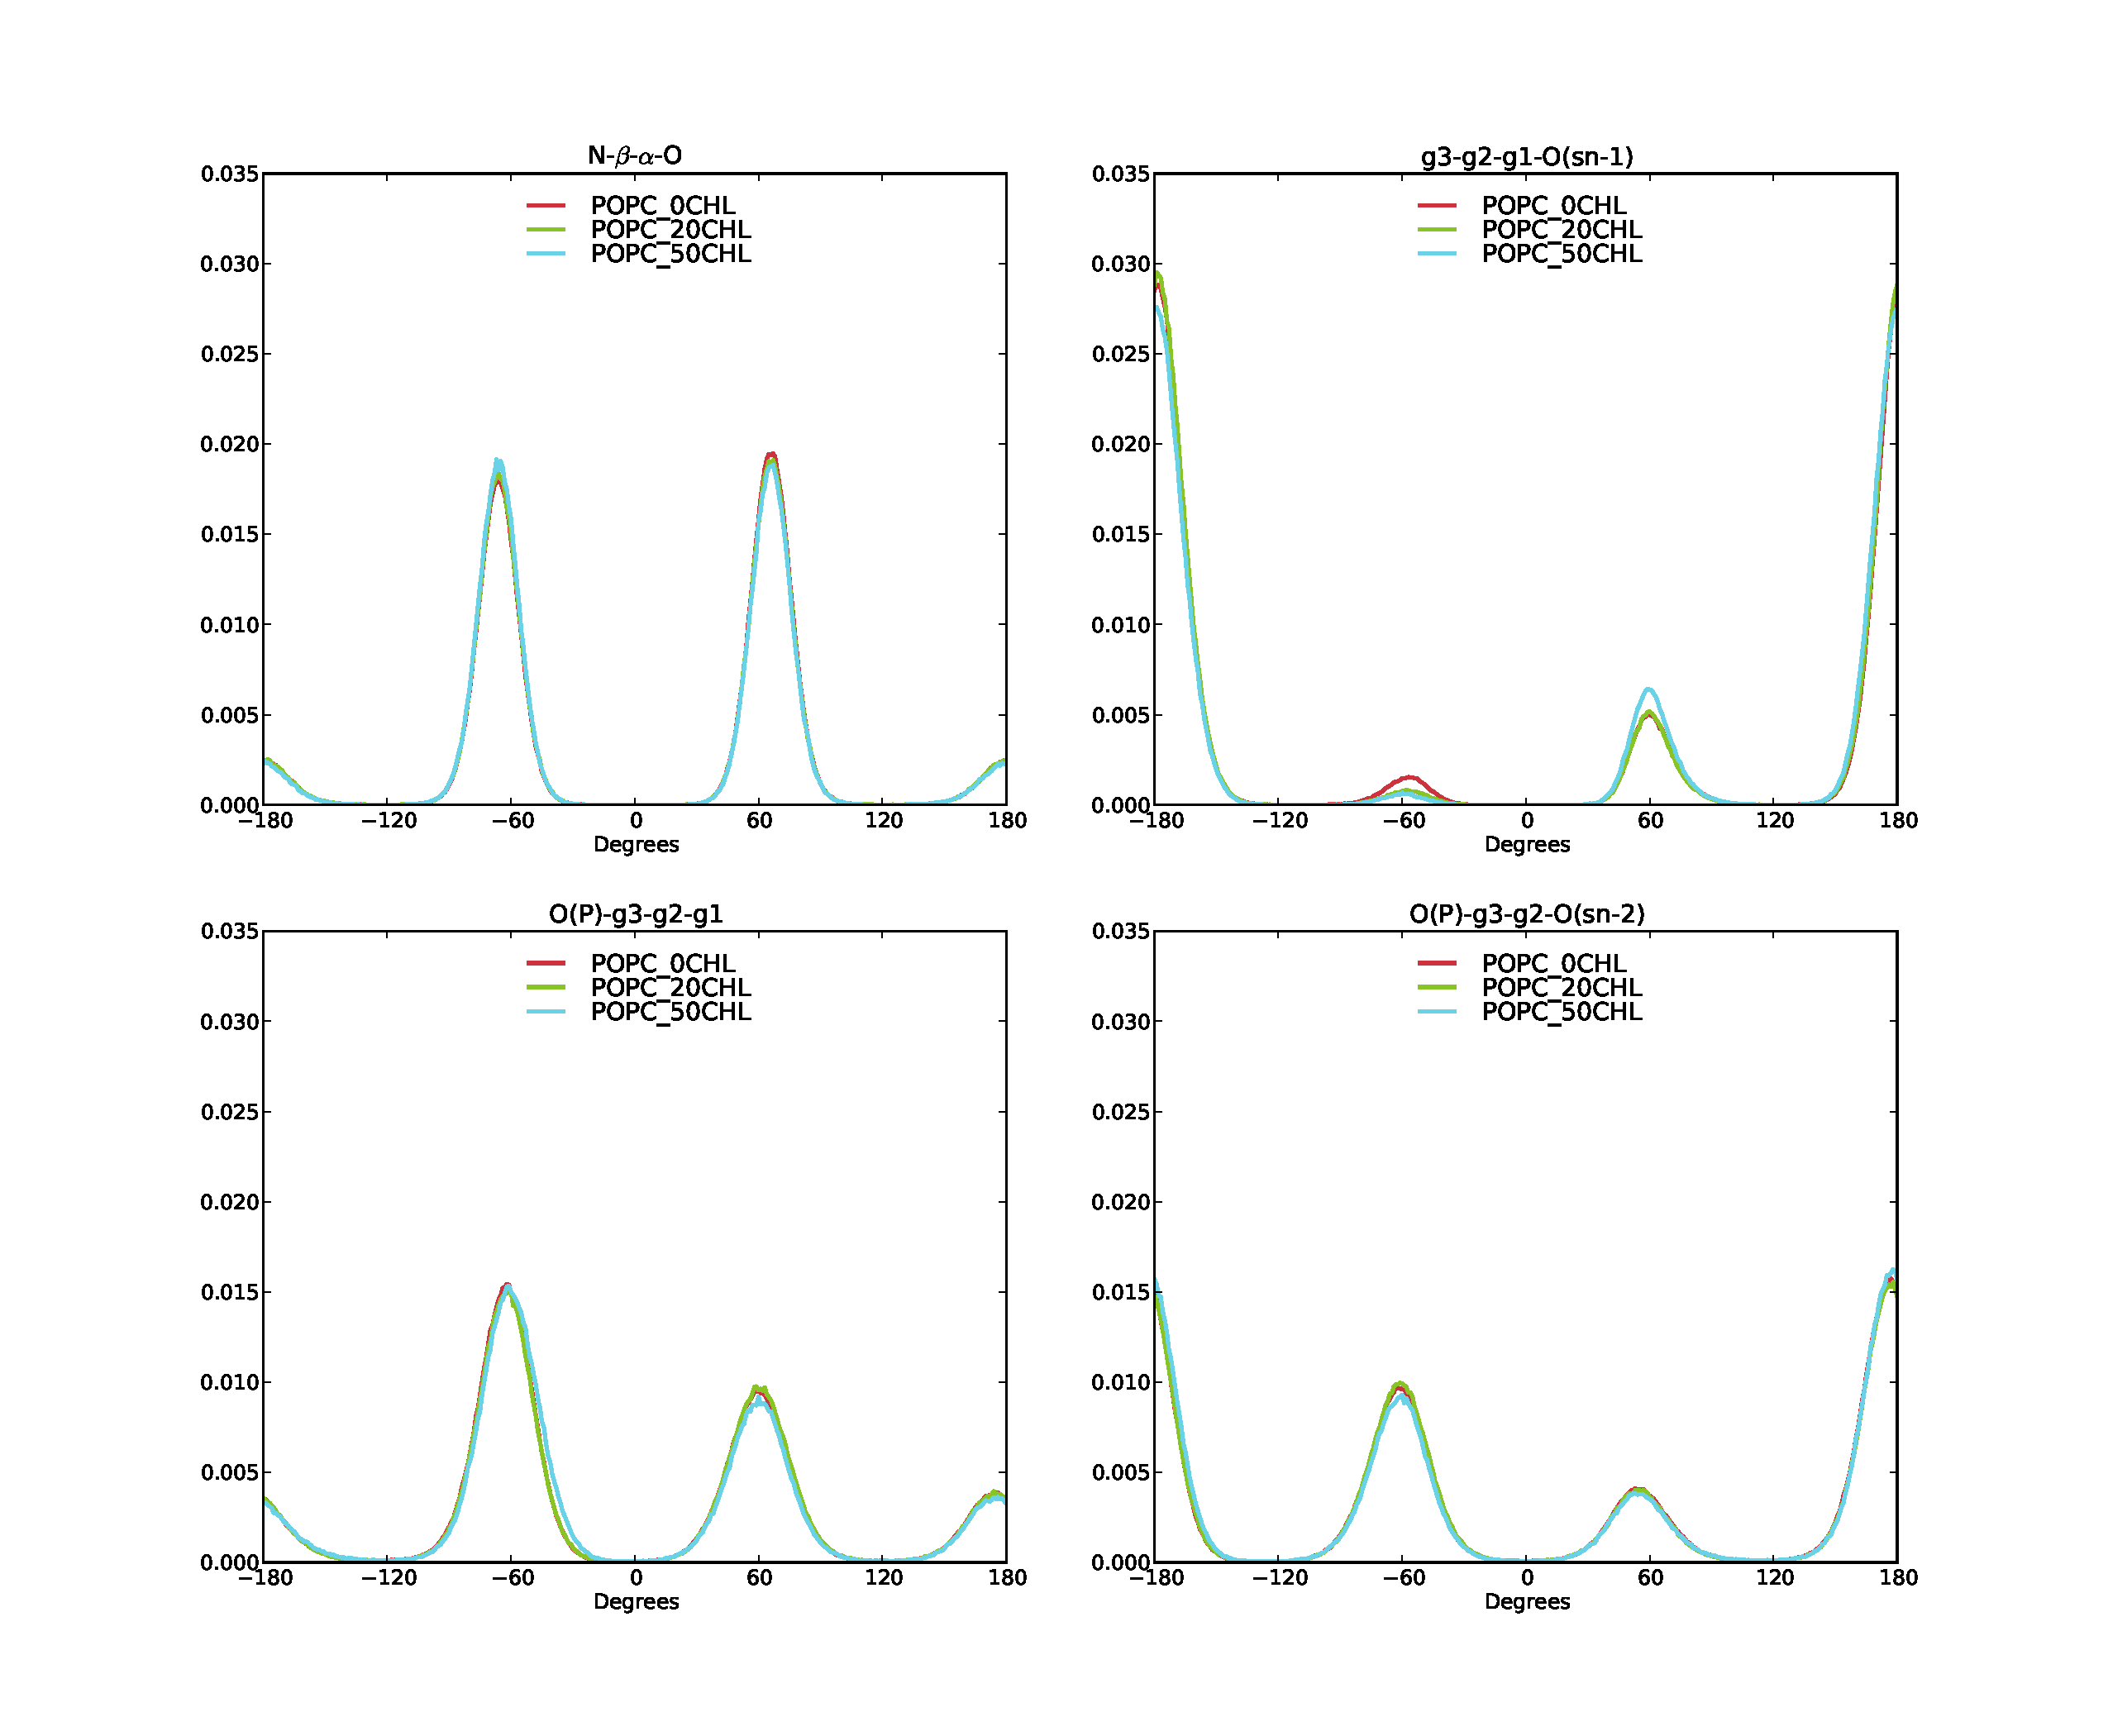
\includegraphics[width=17.2cm]{../Fig/dihsCHOLcharmm.pdf}
  \caption{\label{dihsCHOLcharmm}
    The effect of cholesterol content on the POPC glycerol backbone and choline dihedral angles in CHARMM36 model (T=303~K).}
\end{figure*}

\subsection{Author Contributions}
\todo{Please write a text summarizing your contribution} \\
{\it Alexandru Botan} provided simulation results for charmm36-UA\\
{\it Fernando Favela} prepared, performed and analyzed simulations
with popc and cholesterol for the CHARMM36 All-Atom FF. \\
{\it Patrick F. J. Fuchs} Ran and analyzed the Poger simulations. Provided scientific information which significantly advanced the project (signs and forking of order parameters). \\
{\it Matti Javanainen} prepared and performed simulations with multiple lipid models and analyzed the results. Supervised the work of JT.\\
{\it Matej Kanduc} provided simulation results for the Berger DLPC model \\
{\it Waldemar Kulig} prepared the MD simulations with cholesterol for the MacRog FF \\
{\it Antti Lamberg}  \\
{\it Claire Loison} provided simulation results for charmm36-UA \\
{\it Markus S. Miettinen}  \\
{\it Luca Monticelli}  \\
{\it Jukka M{\"a}{\"a}tt{\"a}}  prepared and performed simulations with Berger and Slipids models and analyzed the results.\\
{\it O. H. Samuli Ollila} Designed and managed the work. Ran and analyzed several simulations. Wrote the manuscript.  \\
{\it Marius Retegan} Prepared and validated the GROMACS compatible parameter files for GAFFlipid and Lipid14 force fields.\\
{\it Tomasz Rog}  \\
{\it Hubert Santuz} prepared and performed the cholesterol simulations with CHARMM36 and analyzed the results. \\
{\it Joona Tynkkynen} prepared and performed the dehydration simulations with the MacRog FF.\\

%\subsection{General issues to think of about the manuscript}
%\todo{Maybe we should mention that CHARMM is significanlty more computationally expensive than other all-atom models.
%This seems evident for a person who has ran CHARMM and other all-atom models with the same computer. However, there
%may be some people who have never used any other model than CHARMM. In this case it may be difficult to realize.
%Would anyone have a good bencmark about this? I have assumed that the reason for the slowness are the extra Lennart-Jones
%interactionsi in water, however, I have never looked into it. Would someone have some hard facts on this?}

%\newpage

\bibliography{refs}

\end{document}
